\documentclass[a4j,12pt,dvipdfmx]{ujreport}
\usepackage[dvipdfmx]{graphicx}
\usepackage{subfigure} %図に(a)(b)(c)と記号を振れるパッケージ
\usepackage{lscape}
\usepackage{hhline}
\usepackage{master}
\usepackage{epsfig}

\usepackage{enumerate}
\usepackage{amsmath}
\usepackage{relsize}
\usepackage{amssymb}

\usepackage[utf8]{inputenc}
\usepackage{atbegshi}
\usepackage{algorithm}
\usepackage{algpseudocode}
\usepackage{url}
\usepackage{colortbl}
\usepackage{booktabs}
\usepackage{longtable}
\usepackage{dcolumn}
\usepackage{bigstrut}
\AtBeginShipoutFirst{\special{pdf:tounicode  UTF8-UCS2}}

% \usepackage{amsmath}
% \usepackage{txfonts}

\setlength{\headsep}{1.1cm}
\textheight=22.5cm
%====[ プリアンプル ]================================================
\begin{document}
\renewcommand{\contentsname}{目 次}
\renewcommand{\thefootnote}{\fnsymbol{footnote}}
\renewcommand{\bibname}{参考文献}

%====[ 表紙 ]========================================================
\pagenumbering{roman}

\begin{titlepage}
\vspace*{0.5cm}
\begin{center}
\LARGE\bf
平成28年度\hspace{1cm}修士論文\\
\end{center}
\vspace{1cm}
\begin{center}
\LARGE\bf{圧縮ベースパターン認識に有用な新しい特徴量の抽出%タイトルを入れる
}
\end{center}
\vspace{1cm}
\begin{center}
\Large

\vspace{0.5cm}
電気通信大学大学院 情報システム学研究科\\
情報システム基盤学専攻\\

\vspace{1cm}

\LARGE
1553003 \hspace{0.3cm} 内野 太智

\vspace{1cm}
\Large
指導教員\\
古賀 久志 准教授\\
南 泰浩 教授\\
新谷 隆彦 准教授\\

\vspace{1cm}
平成29年1月26日
\end{center}
\end{titlepage}


\clearpage

%====[ 目次 ]========================================================
\pagenumbering{roman}
\tableofcontents
\pagebreak
\pagenumbering{arabic}

\def\thline{\noalign{\hrule height 1pt}}
\def\tvline{\vrule width 1pt}
%====[ 本文 ]========================================================
\chapter{序論}
\section{研究背景と研究目的} % (fold)
\label{sec:研究背景と研究目的}


多様な新しい種類のデータが大量に生成されるビッグデータの時代において,データを人手によらないで分類/認識する汎用的なパターン認識手法の重要性が高まっている.
しかし,一般的な統計的パターン認識手法では,パラメータ選択を含めモデルを人手で適切に設計する手間が大きく,新種のデータを分析するのは容易ではない.
これに対して,圧縮ベースパターン認識は,データ圧縮アルゴリズムを用いたパラメータフリーなパターン認識手法であり,1次元に表現されたデータであれば何でも解析可能な汎用手法であるため,近年盛んに研究されている.

圧縮ベースパターン認識は(1)圧縮後のファイルサイズを利用する手法と(2)圧縮時に生成される辞書(以下,
圧縮辞書)から特徴抽出する手法に大別される.
前者の例としては,2つのデータ$x,y$を結合したファイルを圧縮しそのサイズから,$x$と$y$の距離を測る Normalized Compression Distance (NCD) \cite{NCD} が
広く知られている.
また,与えられたデータを複数の辞書で圧縮し,それぞれの辞書で求められた圧縮率を並べて特徴ベクトルとするPattern Representation on Data Compression(PRDC) \cite{PRDC} もよく用いられる.
後者の例としては,LZW圧縮で生成される辞書をデータの要約とみなし,辞書間で類似度を計算する Normalized Dictionary Distance (NDD) \cite{NDD}や単語の多重度も考慮したNormalized Multiset Distance (NMD) \cite{NMD}が提案されている.

本研究は,圧縮ベースパターン認識に有用な特徴の探求を目的とする.具体的には,従来手法であるPRDCとNMDを取り上げ,PRDCに対しては圧縮後のファイルから,NMDに関しては圧縮辞書からそれぞれ新しい特徴を抽出することで,認識精度を向上できることを示す.

また,新しい特徴を抽出する際,特に考慮した点は以下の2つである.
\begin{itemize}
	\item 類似度計算におけるパラメータを増やさない
	\item 特徴抽出のために複雑な計算をしない
\end{itemize}
これにより,圧縮ベースパターン認識の特徴である手軽さを損なわず,実用的な手法の提案を目的とした.

% section 研究背景と研究目的 (end)

\section{本論文の構成} % (fold)
\label{sec:本論文の構成}
以下に本論文の構成を述べる.

\begin{description}
	\item{第2章} 本研究で用いる圧縮アルゴリズムであるLZWの説明と,圧縮ベースパターン認識の代表的な2種類の手法について述べる.
	\item{第3章} 圧縮後のファイルから特徴抽出を行う手法であるPRDCに着目し,圧縮後のファイルから別の特徴を新たに抽出することでPRDCの改良を行う.
	\item{第4章} 圧縮辞書から特徴抽出を行う手法である NMD を取り上げ,圧縮辞書からの新しい特徴抽出による NMD の改良手法を説明する.
	\item{第5章} 本研究で提案した手法の評価実験を画像と時系列データに対して行い,その有効性を示す.
	\item{第6章} 本研究のまとめと今後の課題について述べる.
\end{description}
% section 本論文の構成 (end)
\chapter{圧縮ベースパターン認識}
% 本章では,既存の圧縮ベースパターン認識手法を紹介する.
本章では,はじめに圧縮ベースパターン認識で利用される圧縮アルゴリズムである,LZWについて説明し,
その後,圧縮後のファイルサイズを利用する手法と圧縮辞書から特徴抽出する手法それぞれについて述べる.


\section{LZW圧縮アルゴリズム}
この章では,本研究でオブジェクトの符号化と辞書の作成に用いる,LZW圧縮アルゴリズムについて詳しく述べる.
LZWでは,高速かつ高い圧縮効率を追求しており,現在もGIF画像やTIFF画像などの圧縮に用いられている圧縮アルゴリズムである.

LZW符号化の手順について説明する.
符号化では,圧縮されたテキストと復号に用いられる辞書が得られるが,
本研究ではこの辞書を利用している.なお,ここでは
圧縮元のテキストは8bitの記号を前提として説明する.

\begin{table*}[tb]% Table 1
\caption{初期状態のLZW辞書.}
%\ecaption{Comparison of correlation coefficient between baseline(upper right) and proposed(lower left) method(bold letter indicate  that absolute value of  correlation coefficient is less than 0.4 in the cell).}
\label{lz}
\begin{center}
\scalebox{1}{
\begin{tabular}{r|r  }
\hline
単語 & 符号 \\
\hline
(0) & 0 \\
(1) & 1 \\
\vdots & \vdots \\
(255) & 255 \\
\hline
\end{tabular}%
}
\end{center}
\end{table*}

\begin{description}
	\item [Step1] 8bitの256種類の全記号を登録した辞書を用意する.ここで,記号を8bitの整数として扱った場合の整数値をその単語の符号とする(表\ref{lz}).
	さらに,最長一致文字列とその符号を記憶する領域(バッファ)を確保する.

	\textgt{
	バッファの状態:最長一致文字列 = (空),符号 = (空)
	}
	\item [Step2] テキストの最初の記号を読み込んで最長一致文字列とし,
	それを整数として扱った値を符号として記憶する.
	例えば最初の記号が'a'で,その整数値が97とするとバッファの内容はつぎのようになる.

	\textgt{
	バッファの状態:最長一致文字列 = a,符号 = 97
	}
	\item [Step3] 次の記号を読み込み,その記号を最長一致文字列に
	追加した「現在の最長一致文字列+読み込んだ記号」という単語を
	辞書から探して,以下のいずれかの処理をおこなう.
	\begin{description}
		\item [(a)単語が辞書にある]
		その単語を最長一致文字列にして,その符号を記憶する.
		この操作を,「現在の最長一致文字列+読み込んだ記号」が辞書にない記号列になるまで繰り返す.
		\item [(b)単語が辞書にない]現在の最長一致文字列の符号を出力し,記号列を新しい単語として辞書に登録する.Step4へ.
	\end{description}
	例えばバッファの状態がつぎのようになっているとする.

	\textgt{
	バッファの状態:最長一致文字列 = c$\cdots$b,符号 = 312
	}

	このとき,次に読み込んだ記号を'c'として「c$\cdots$bc」が辞書にない場合,
	現在の最長一致文字列c$\cdots$bの符号を出力する($312_{(10)}$ = $100111000_{(2)}$).そして,記号列c$\cdots$bcを新しい単語として辞書に登録
	する.仮に,記号列c$\cdots$bcの符号を410とすると,登録後の辞書は
	表\ref{lz2}のようになる.

	\item [Step4] 今読み込んだ記号をあらためて最長一致文字列として,その整数値の符号を記憶する.前のステップの例をそのまま用いると,バッファの状態はつぎのようになる.

	\textgt{
	バッファの状態:最長一致文字列 = c,符号 = 99
	}

	\item [Step5] オブジェクト列が終了するまで,Step3$\sim$Step4を繰り返す.

\end{description}

\begin{table*}[tb]% Table 1
\caption{単語を登録した後のLZW辞書.}
%\ecaption{Comparison of correlation coefficient between baseline(upper right) and proposed(lower left) method(bold letter indicate  that absolute value of  correlation coefficient is less than 0.4 in the cell).}
\label{lz2}
\begin{center}
\scalebox{1}{
\begin{tabular}{r|r  }
\hline
単語 & 符号 \\
\hline
(0) & 0 \\
(1) & 1 \\
\vdots & \vdots \\
(255) & 255 \\
\vdots & \vdots \\
c$\cdots$b & 312 \\
\vdots & \vdots \\
c$\cdots$bc & 410 \\
\hline
\end{tabular}%
}
\end{center}
\end{table*}



\section{圧縮後のファイルサイズを利用する手法}
\subsection{基本的な考え}
%中島先輩の論文から引用
現在用いられている,圧縮後のファイルサイズ(圧縮率)を用いた手法の基本となる
概念はコルモゴロフ複雑性(Kolmogorov Complexity)\cite{osamu2006}が基となっている.
コルモゴロフ複雑性は,有限長のオブジェクト列の複雑度を表す指標であり,
与えられた文字列$x$に対してのコルモゴロフ複雑性$K(x)$はつぎのように定義される.
\begin{equation}
K(x) = \min_{q \in Q_x} |q| \label{kol}
\end{equation}
これは文字列$x$を出力可能なプログラム集合$Q_x$において,
この中で最小の文章量をもつプログラム$q$の長さが$K(x)$となる.
この値が大きいほど,その文字列は複雑と解釈される.

例として,つぎの2つの入力文字列を考える.
\begin{verbatim}
文字列1:xwxwxwxwxwxwxwxwxwxw
文字列2:3s2sm6br4z2f9cfd8jza
\end{verbatim}
これらの文字列を出力するプログラムを考えた時,
前者は「xwを10回出力」に対し,後者は
特に規則性をもたないので「3s2sm6br4z2f9cfd8jzaを出力」
と書く他はないように思える.
この場合,文字列を出力するプログラムの長さは後者のほうが長いので,
文字列2は文字列1より複雑であると考えられる.このようにコルモゴロフ複雑性では,
文字列を説明するプログラムの長さは,文字列そのものの複雑さと関係していることを
示している.

以上で説明した式(\ref{kol})は,プログラムが単独で$x$を生成する場合の定義である.
さらに,$y$に対する$x$の相対的コルモゴロフ複雑性を$K(x|y)$をつぎのように定義する.
\begin{equation}
K(x|y) = \min_{q(y) \in Q_x} |q(y)| \label{kol2}
\end{equation}
これは,$y$という補助オブジェクトを入力として,$x$を生成する
プログラムの最小長である.
一般的に,$y$に含まれる情報を用いる場合はより短いプログラムで$x$
が生成できる.したがって,$K(x|y)$は$K(x)$よりも小さくなる可能性がある.
この時に$K(x)$,$K(x|y)$の差$K(x)-K(x|y)$は,
$x$を予備知識なしに圧縮する場合に対し,$y$を仮定して
圧縮する場合の「改善度」を表す.すなわち,$K(x)-K(x|y)$は
$x,y$両者の類似部分の量と解釈することができる.

以上に説明したコルモゴロフ複雑性は計算不能として知られており,実際に
は用いることはできない.
そこで実用的には,データ圧縮技術を用いてオブジェクトの情報量や
オブジェクト間の類似性を評価している.

オブジェクト自身の複雑度を評価する場合は,そのオブジェクトを圧縮した時の
圧縮率で判断する.ただし,圧縮率はつぎのように定義される.
\begin{equation}
圧縮率 = \frac{圧縮後のファイルのサイズ}{圧縮前のファイルのサイズ}
\end{equation}
以上の定義から,圧縮率が大きい場合はそのオブジェクトの圧縮効率が悪いことが分かる.
つまり,圧縮率が大きい場合はオブジェクトは複雑であり,小さい場合はオブジェクトは単純
であると解釈できる.

例として,先ほど挙げた2つの文字列をUNIX標準のcompressコマンド
によって圧縮した結果を示す.

\begin{verbatim}
文字列1:xwxwxwxwxwxwxwxwxwxw を圧縮した場合
~$compress -f -v string1.txt
string1.txt:  -- replaced with string1.txt.Z Compression: 33.33%
文字列2:3s2sm6br4z2f9cfd8jza を圧縮した場合
~$compress -f -v string2.txt
string2.txt:  -- replaced with string2.txt.Z Compression: -28.57
\end{verbatim}
なお,出力におけるCompressionは圧縮効率(何\%削減できたか)を表す.
結果を見ると,文字列1は規則的なパターンをもつ単純な文字列なので,
圧縮ができていることがわかる.対して,文字列2は不規則なパターンをもつ
文字列であり,圧縮が上手くできておらず圧縮前よりもサイズが上回っていることがわかる.
このように,コルモゴロフ複雑性と同様に,テキストの複雑さとその圧縮率には関係性があり,
データ圧縮によって評価できることが分かる.

つぎにデータ圧縮技術によってオブジェクト間の類似度を評価する考え方について説明する.
オブジェクト$x,y$が似ているかどうか調べる場合,まずオブジェクト$y$の情報を用いて
,もう一方のオブジェクト$x$の圧縮をおこなう.
$y$の情報を用いて$x$を圧縮する処理は,具体的には
はじめに$y$を圧縮することで得られる辞書を作成する(図\ref{dic}).

\begin{figure}[tb]
\begin{center}
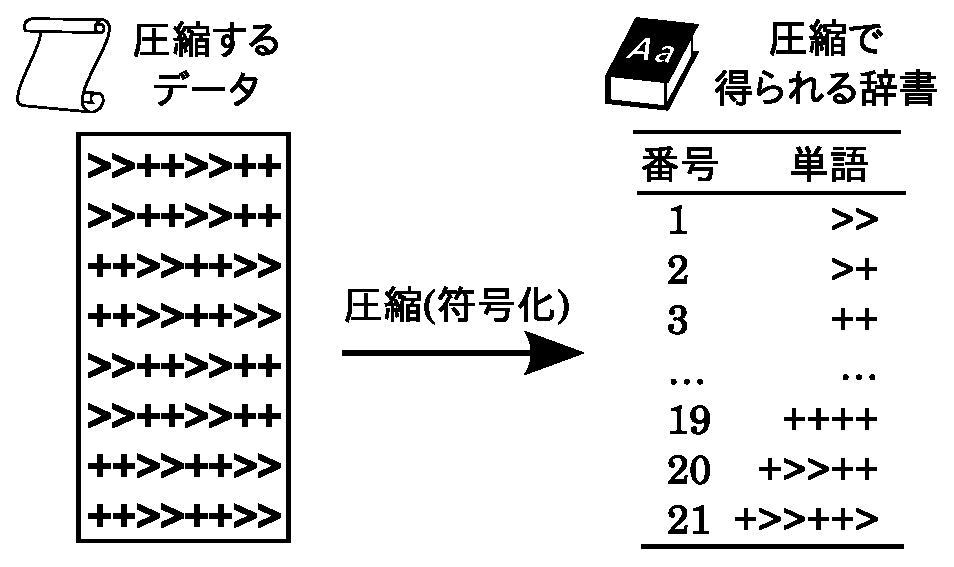
\includegraphics[width=10.5cm]{image/dic.eps}
\end{center}
\caption{データ圧縮によって得られる辞書.}
\label{dic}
\end{figure}
この辞書は圧縮対象のオブジェクトに頻出するパターンを保持していることがわかる.
そしてこの$y$の辞書を用いて,$x$を圧縮することで圧縮率を求める.
この圧縮率が
大きい場合には,$y$は$x$と類似するパターンを持っていないので,似ていないと解釈できる.
逆に圧縮率が小さい場合には,$y$は$x$と類似するパターンを多く持っているため,
似ていると解釈できる.

まとめると,オブジェクトに対する圧縮率の大小はつぎのように定義できる.
\begin{description}
	\item [圧縮率が大きい] オブジェクトのランダム性が高い $\Rightarrow$ 複雑なオブジェクト
	\item [圧縮率が小さい] オブジェクトのランダム性が低い $\Rightarrow$ 単純なオブジェクト
\end{description}
以上がデータ圧縮技術を用いた,オブジェクトの解析方法である.


\subsection{Normalized Compression Distance(NCD)}
\label{subsec:NCD}

NCD \cite{NCD} は2つのオブジェクト$x,y$間の距離を圧縮後のファイルサイズから算出する手法である.
$x,y$間の距離 NCD($x,y$)は式\ref{eq:NCD}のように定義される.
\begin{eqnarray}
\mathrm{NCD}(x,y) = \frac{C(xy) - \min\{C(x),C(y)\}}{\max\{C(x),C(y)\}} \label{eq:NCD}
\end{eqnarray}
ここで$C(x)$はオブジェクト$x$を圧縮したときのファイルサイズ,また$C(xy)$はオブジェクト$x,y$を連結した
$xy$を圧縮したときのファイルサイズを表す.$x,y$が類似しているほど$xy$がよりコンパクトに圧縮できるので,
$\mbox{NCD}(x,y)$は小さくなる.

NCDでは,図\ref{ncd}のようにオブジェクト$x$と$y$で共通するパターンが
多い場合に$C(xy)$は小さくなる.対して,$x$と$y$で共通するパターンが
少ない場合には$C(xy)$は大きくなる.このような性質を持っている.

\begin{figure}[tb]
\begin{center}
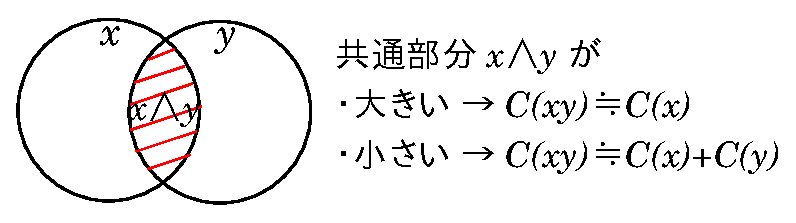
\includegraphics[width=13.5cm]{image/ncd.eps}
\end{center}
\caption{NCDの性質.}
\label{ncd}
\end{figure}

式(\ref{eq:NCD})から分かるように,NCDは計算において,パラメータを必要としない
パラメータフリーな手法といった利点がある.
しかし,NCDでは類似度の計算の度に$xy$の圧縮計算が必要である.
仮に文字列$x$,文字列$y$の文字数をそれぞれ$n_x, n_y$とし,
$x$から抽出される辞書の単語数を$m_x$,$y$から抽出される辞書の単語数を$m_y$として,$C(xy)$の計算量を考える.
なお,辞書の単語は辞書式順にソートされているとする.
このとき,オブジェクト$xy$の圧縮を考えると,最大でサイズが$m_x + m_y$の辞書に対して二分探索を
して単語を探す操作を,$n_x + n_y$回おこなう必要がある.
したがって,$C(xy)$の計算量は$(n_x + n_y)\log(m_x + m_y)$と表せる.

NCDをデータ集合の分類に適用した場合,データペア間の距離行列の計算が必要である.
この距離行列の計算量はデータベースに登録されているデータ数の2乗オーダとなる.
この為NCDでは,データの数が100個を超えるようなデータセットへの適用が難しい
という問題がある.




\subsection{PRDC}
PRDC \cite{PRDC} では,圧縮率ベクトルと呼ばれる特徴量によりオブジェクトを表現して,分類や類似検索を実現する.
PRDCはオブジェクトを特徴ベクトルとして扱うので,NCD等の距離尺度と比べると,$k$-means法や
SVM(Support Vector Machine)などベクトルベースのパターン認識手法の利用に適する.

PRDCでは,$N$個の基底辞書集合$B=\{D_1,D_2,\dots,D_N\}$を最初に定める.そして,オブジェクト$x$を
それぞれの辞書で圧縮した$N$次元の圧縮率ベクトルとして$x$を表現する.(図\ref{fig:PRDC.eps})
\begin{figure}[tb]
\centering
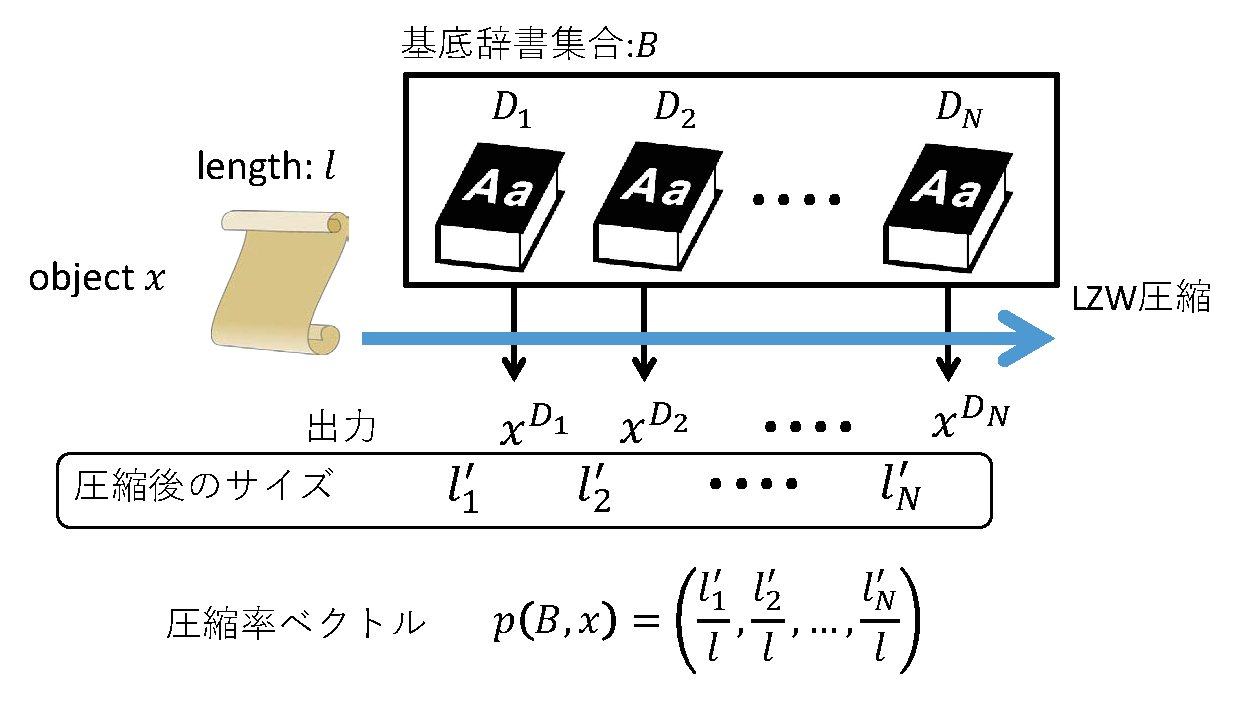
\includegraphics[clip, width=\columnwidth]{image/PRDC.eps}
\caption{圧縮率ベクトルの作成}
\label{fig:PRDC.eps}
\end{figure}

圧縮率ベクトル$\boldsymbol{p}(B,x)$はつぎのように定義される.

\begin{equation}
\boldsymbol{p}(B,x) = \biggl(\frac{l'_1}{l}, \frac{l'_2}{l},\dots,\frac{l'_N}{l} \biggr).
\label{eq:PRDC}
\end{equation}
長さ$l$の入力オブジェクト$x$が与えられた時,$x$をそれぞれの基底辞書により圧縮すると,
出力長$l'_1,l'_2,\dots,l'_N$が得られる.それぞれの出力長を元のオブジェクト長$l$で割った圧縮率を
並べたのが圧縮率ベクトルとなる.ここで出力長とは圧縮後のファイルサイズに他ならず,
PRDCも圧縮後のファイルサイズを利用する手法と位置づけられる.

\begin{figure}[tb]
\begin{center}
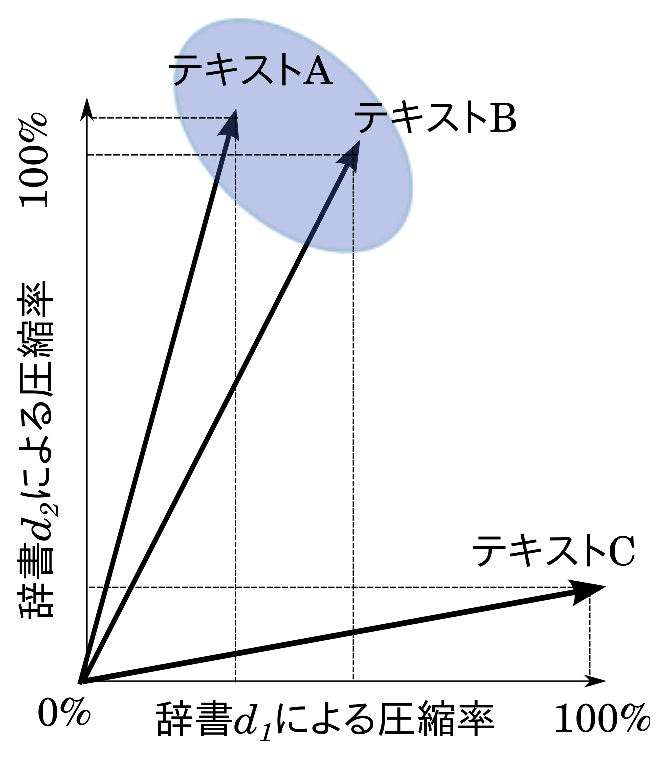
\includegraphics[width=8.5cm]{image/cv.eps}
\end{center}
\caption{圧縮率ベクトルによるテキストの特徴表現.}
\label{cv}
\end{figure}

例えば,図\ref{cv}のようにA,B,Cというオブジェクトがあった場合,2つの圧縮辞書$d_1$と$d_2$
を用いてそれらオブジェクトの特徴を2次元の圧縮率ベクトルで数値化し,
圧縮率ベクトル空間に写像する.
ここで空間上のベクトル間の距離に着目すると,AはCよりもBのほうが近い
位置にあるので,Bに対してAはCよりも似ていると言える.
PRDCではこのように,データ圧縮技術を用いて様々なファイルを特徴づける.

%つまり,$\boldsymbol{p}(D,x)$は入力テキスト$x$を基底辞書集合$D$によって圧縮して得られる
%ベクトルを表す.
%このようにPRDCでは元のオブジェクトを数値ベクトルとして表現し,

ここで,基底辞書集合$B=\{D_1,D_2,\dots,D_N\}$は,データベースから選択した$N$個のオブジェクト群
$\{T_1,T_2,\dots,T_N\}$を実際に圧縮して生成する.どのオブジェクトを利用するかはパターン
認識性能に影響を与える因子である.\cite{PRDC}では,以下のような基底辞書集合の生成方法を
提唱している.まず,$N$個のオブジェクトをランダムに選んで暫定的な圧縮特徴空間を構築する.
そして,暫定特徴空間上でデータベース内のオブジェクトをクラスタリングし,クラスタ代表となった
$N$個のオブジェクトから最終的な基底辞書集合を生成する.

%例えば,A,Bの2つのオブジェクトがあり,Aから作られた辞書を用いて,Bを圧縮した場合,
%それが高圧縮であればAとBは似ていると考えられる.

%ここであらかじめ様々な種類のテキスト群$T=\{t_1,t_2,\dots,t_N\}$を収集しておき,
%それを圧縮することによって得られる辞書群$D=\{d_1,d_2,\dots,d_N\}$を基底辞書集合とする.
\section{辞書に基づく非類似度計算}
\ref{subsec:NCD}章で述べたNCDでは類似度を算出する際に毎回オブジェクトを圧縮するために,類似度計算の計算量が
大きい.そこで,図\ref{fig:image/Create_dictionary.eps}のように,予めオブジェクトを圧縮し,その過程で構成された圧縮辞書をオブジェクトの要約とみなし,その辞書間で距離(非類似度)を計算する手法が提案された.
圧縮アルゴリズムとしてはLZWが利用される.

\begin{figure}[tb]
\begin{center}
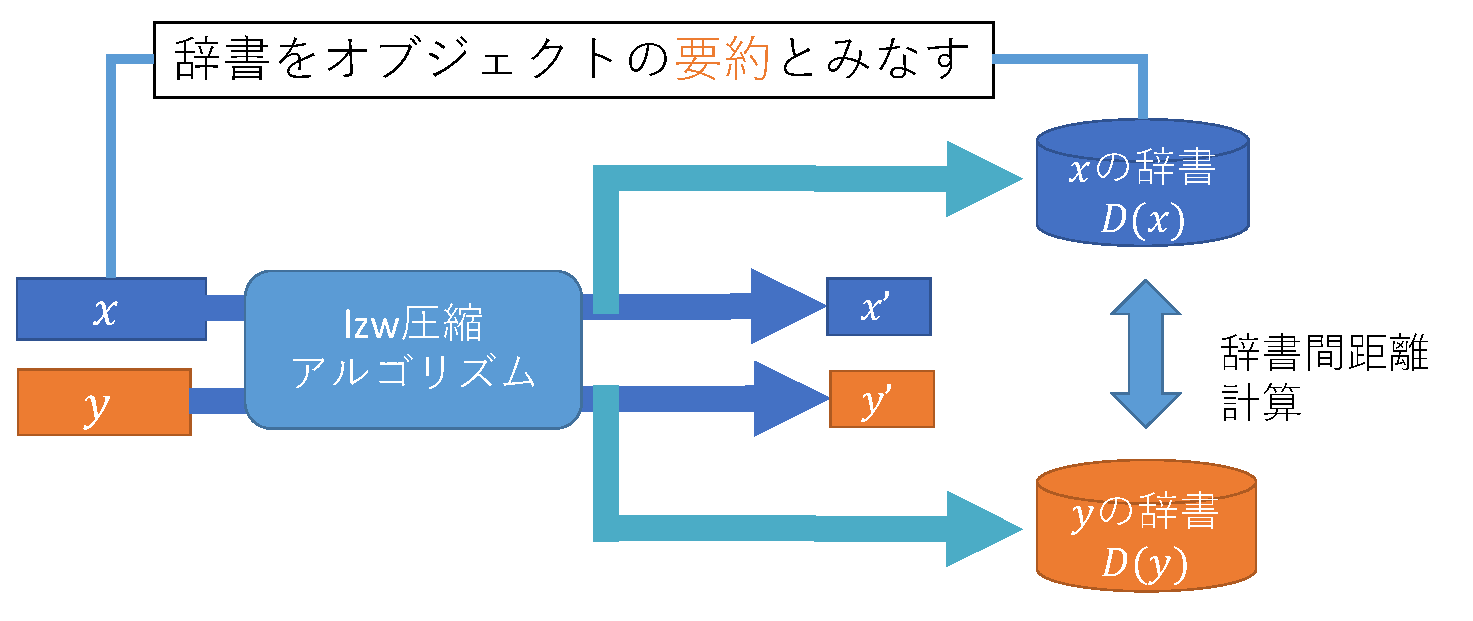
\includegraphics[clip, width=\columnwidth]{image/Create_dictionary.eps}
\caption{辞書に基づく非類似度(距離)計算}
\label{fig:image/Create_dictionary.eps}
\end{center}
\end{figure}



% LZWによる辞書構築の流れを図~\ref{fig:image/lzw.eps}に示す.
% LZWアルゴリズムによる辞書の構築は,次の手順で行う.
% 辞書には,長さ1の全ての文字が単語として登録されているものとする.
% \begin{enumerate}
% 	\item 辞書から,入力文字列に存在する最も長い単語Wを探す.
% 	\item 入力文字列中の単語WをWの符号に置き換える.
% 	\item 辞書に,入力文字列中のWとその次の1文字を結合した単語を登録する.
% 	\item 入力文字列中に符号に置き換えられていない文字が存在すれば,1に戻る.
% \end{enumerate}

%圧縮率に基づく類似度計算では,圧縮アルゴリズムにより出力される符号化文字列から特徴量を取り出し,分類を行っている.また,圧縮辞書に基づく類似度計算では,圧縮アルゴリズムにより構成される辞書から特徴量を取り出し,類似度の計算をこなっている.


%辞書に基づく非類似度(距離)計算では,オブジェクトをLZW圧縮アルゴリズムで圧縮
%した際に構成される辞書が利用される.

%辞書構築の全体的な流れは
%図\ref{fig:image/lzw.eps}のようになる.まずオブジェクトから文字列を作成する.
%オブジェクトから文字列を作成する例として,画像処理でよく用いられる方法に,水
%平スキャンがある.
%これは画像の左側から右側へ水平方向に走査し,ピクセル
%の情報を文字列に変換する方法である.

\subsection{NDD} % (fold)
\label{sub:ndd}

% subsection ndd (end)
辞書による非類似度の例としては,Normalized Dictionary Distance (NDD) \cite{NDD} がある.
NDDでは,辞書を登録された単語の集合として取扱う.$D(x)$をオブジェクト$x$に対する
圧縮辞書とする.$x,y$間の距離 NDD($x,y$)は式(\ref{eq:NDD})のように定義される.
\begin{eqnarray}
\mathrm{NDD}(x,y) = \frac{ \cup(D(x),D(y)) - \min\{|D(x)|,|D(y)|\} }{ \max\{|D(x)|,|D(y)|\} }
\label{eq:NDD}
\end{eqnarray}
$|D(x)|$は$D(x)$に含まれる単語数,$\cup(D(x),D(y))$は$D(x)$と$D(y)$の和集合である.
2つの辞書が共通単語を多く含むほど$\cup(D(x),D(y))$の要素数が小さくなり,辞書間距離は小さくなる.

\subsection{NMD} % (fold)
\label{sec:nmd}
% section nmd (end)
辞書間距離の本質は,辞書を元オブジェクトの要約として用いることで計算量を削減することにある.
その一方で,辞書は元オブジェクトから情報を捨てており,この点が辞書間距離の欠点である.
そこで,Besirisらは辞書$D(x)$内の各単語が元オブジェクト$x$内に出現する回数を考慮した
辞書間距離Normalized Multiset Distance (NMD) \cite{NMD}を提案した.NMDでは,図\ref{fig:image/CalcNMD.eps}のように単語の出現回数を考慮した単語の多重集合間で距離計算をする.
ここで多重集合における単語の重複度は,出力における符号の出現回数である.(例外的に,辞書に存在するが出力には出現しない単語は,重複度1として扱う.)
\begin{figure}[tb]
\begin{center}
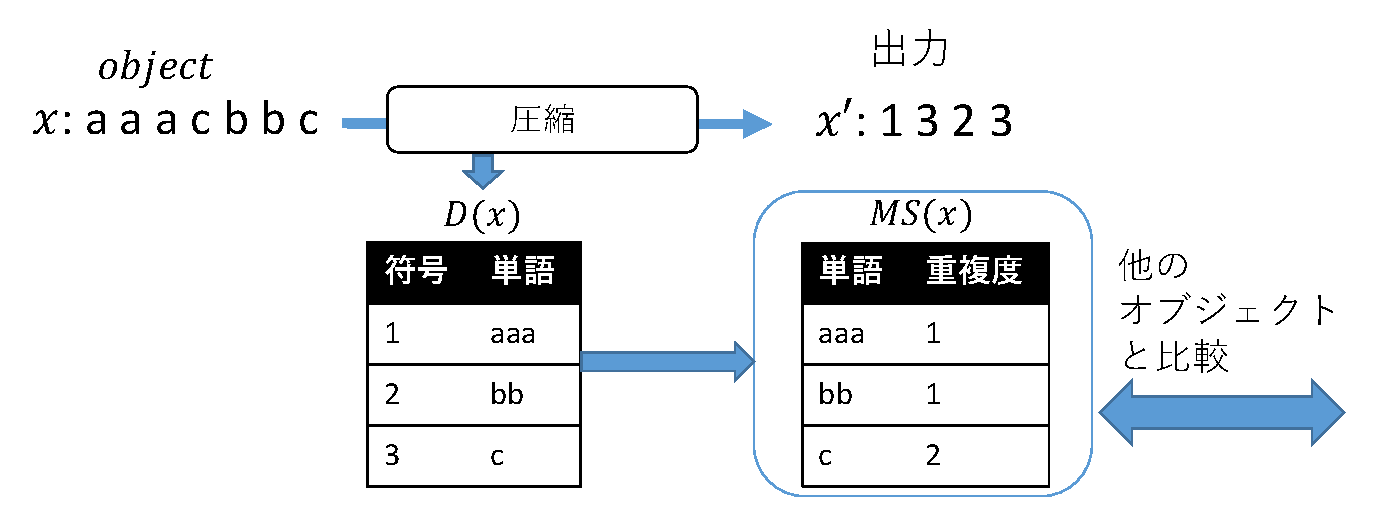
\includegraphics[clip, width=\columnwidth]{image/CalcNMD.eps}
\caption{NMD計算の流れ}
\label{fig:image/CalcNMD.eps}
\end{center}
\end{figure}

文字列$x$の辞書$D(x) = \{w_1,w_2,...,w_n\}$を順序不同の$n$個の単語の集合、$w_i$を$i$番目に抽出された単語としたとき、その多重集合$MS(x)$は次のよう
に定義される。
\begin{align}
MS(x)
&= \{D(x),m^x\} \notag \\
&= \{(w_1,m_1^x),(w_2,m_2^x),...,(w_n,m_n^x)\}
\end{align}
ここで$m_i^x$は$i$番目の単語$w_i$の出現回数であり、$m^x$は$x$中の単語出現回数を並べたリストである.$MS(x)$の要素数$|MS(x)|$は次のように定義される.
\begin{equation}
|MS(x)| = \sum_{i=1}^n m_i^x
\end{equation}

$x,y$間の距離 NMD($x,y$)は式(\ref{eq:NMD})で計算される.
\begin{equation}
\frac{|MS(x)\cup MS(y)| - \min(|MS(x)|,|MS(y)|)}{\max(|MS(x)|,|MS(y)|)}
\label{eq:NMD}
\end{equation}
式$(\ref{eq:NMD})$では,2つの多重集合$MS(x) = \{D(x),m_x\}$, $MS(y) = \{D(y),m_y\} $間で
非類似度を計算する式になっている.$MS(x)$と$MS(y)$の和集合$MS(z)= \{D(z),m_z\}=
MS(x)\cup MS(y)$は
\begin{gather}
\label{eq:x_cup_y_0}
D(z) = D(x)\cup D(y) \\\label{eq:x_cup_y_1}
m_z(w_i) = \max(m_x(w_i),m_y(w_i))
\end{gather}
として定義される。
%これらに基づき、Normalized Multiset Distance(NMD)という非類似度(距離)を以下のように定義する.


%NDDは任意のオブジェクト$x,y$から作成された辞書$D(x),D(y)$に対して次のように定義される.
%\begin{equation}
%NDD(x,y)
%\end{equation}

%\label{sub:nmd}
\cite{NMD}はNDDよりもパターン認識精度を向上させることを示した.

\chapter{High-Order PRDC}
本章では,圧縮後のファイルから特徴抽出を行う手法であるPRDCに着目する.
そして,圧縮後のファイルから別の特徴を新たに抽出することでPRDCを改良する.

まず,PRDCが使用する圧縮率は,テキスト内の単語頻度のみで決定され
異なる単語間の関係を一切利用していない特徴であることを指摘する.そして,隣接
する単語関係を表す新しい特徴量を提案する.その後で新しい特徴量をPRDCに組み込んだ
手法を提案する.

\section{圧縮率} % (fold)
\label{sec:圧縮率}
PRDCが利用する圧縮率について考察する.PRDCではLZWアルゴリズムを用いて,基底辞書$D$に単語とそれに対応する符号(出力記号)
のペアを登録する.符号の長さは元の単語長よりも小さい.そして,圧縮時には入力テキスト$T$を前方からスキャンし,
$T$内の単語を対応する符号に順次置き換えることで圧縮を実現する.
一般に$T$を辞書$D$を使って圧縮した時の圧縮率は
\begin{eqnarray}
圧縮率 &=& \frac{圧縮後のファイルサイズ}{元テキストTのサイズ} \nonumber \\
&=& \frac{圧縮後の符号数 * 1符号の\mbox{bit}長}{Tの文字数 * 1文字の\mbox{bit}長} \nonumber \\
&=& \frac{圧縮後の符号数}{Tの文字数} * \alpha
%&= \frac{\sum_{i=1}^n m_i}{元のテキストの長さ} * \alpha
\label{eq:compress}
\end{eqnarray}
と記述できる.だたし,$\alpha=\frac{1符号の\mbox{bit}長}{1文字の\mbox{bit}長}$を表す定数である.

ここで辞書$D$に$n$種類の単語$(w_1,w_2,..,w_n)$が登録されているとする.単語$w_i$の文字数を$l_i$とおく.
さらに$T$内の単語$w_i$の出現回数を$m_i$と記述する.この時,式(\ref{eq:compress})における
圧縮後の符号数は$\sum_{i=1}^n m_i$である.一方,$T$の長さは$\sum_{i=1}^n m_il_i$になる.
従って,式(\ref{eq:compress})は次のように書き換えられる.
\begin{equation}
\begin{split}
圧縮率 &= \frac{\sum_{i=1}^n m_i}{\sum_{i=1}^n m_i l_i} * \alpha \cr
&= 1-(1-\frac{\sum_{i=1}^n m_i}{\sum_{i=1}^n m_i l_i}) * \alpha \cr
&= 1- \frac{\sum_{i=1}^n m_i(l_i -1)}{\sum_{i=1}^n m_i l_i} * \alpha \cr
&= 1- \frac{\sum_{i=1}^n m_i(l_i -1)}{Tの長さ} * \alpha
\end{split}
\label{eq:ncomp}
\end{equation}
$l_i -1$は$w_i$の符号化1回で削減される文字数であり,$m_i(l_i -1)$は,$w_i$の符号化に
より元のテキストから何文字削減できるかを表す.
式(\ref{eq:ncomp})が示すように圧縮率は各単語の出現頻度のみで決定される特徴量であり,
$T$内における異なる単語の関係は考慮しない.例えば,どの単語とどの単語が$T$内で
隣接して出現するかという情報は圧縮率には反映されない.
%元テキストにおける単語の隣接関係は全く考慮されていない.
% section 圧縮率 (end)

\section{単語の隣接関係を抽出する単純な手法} % (fold)
\label{sec:単語の隣接関係を抽出する単純な手法}
前節で述べたように,基底辞書による圧縮率は$T$に各単語が何回含まれるかによって決定される特徴量であるが,これは$T$内でどの単語が隣接して出現するかという情報を捨ててしまっている.
隣接関係を抽出する単純な方法としては,図~\ref{fig:image/N-Gram.eps}のように,元のオブジェクト列をN-Gramのようにグループ分けし,そのヒストグラムから特徴を抽出する事が考えられる.しかし,この手法ではいくつの符号を1グループにするかという追加のパラメータが必要になり,PRDCを手軽さの面で下回る.

\begin{figure}[tb]
\begin{center}
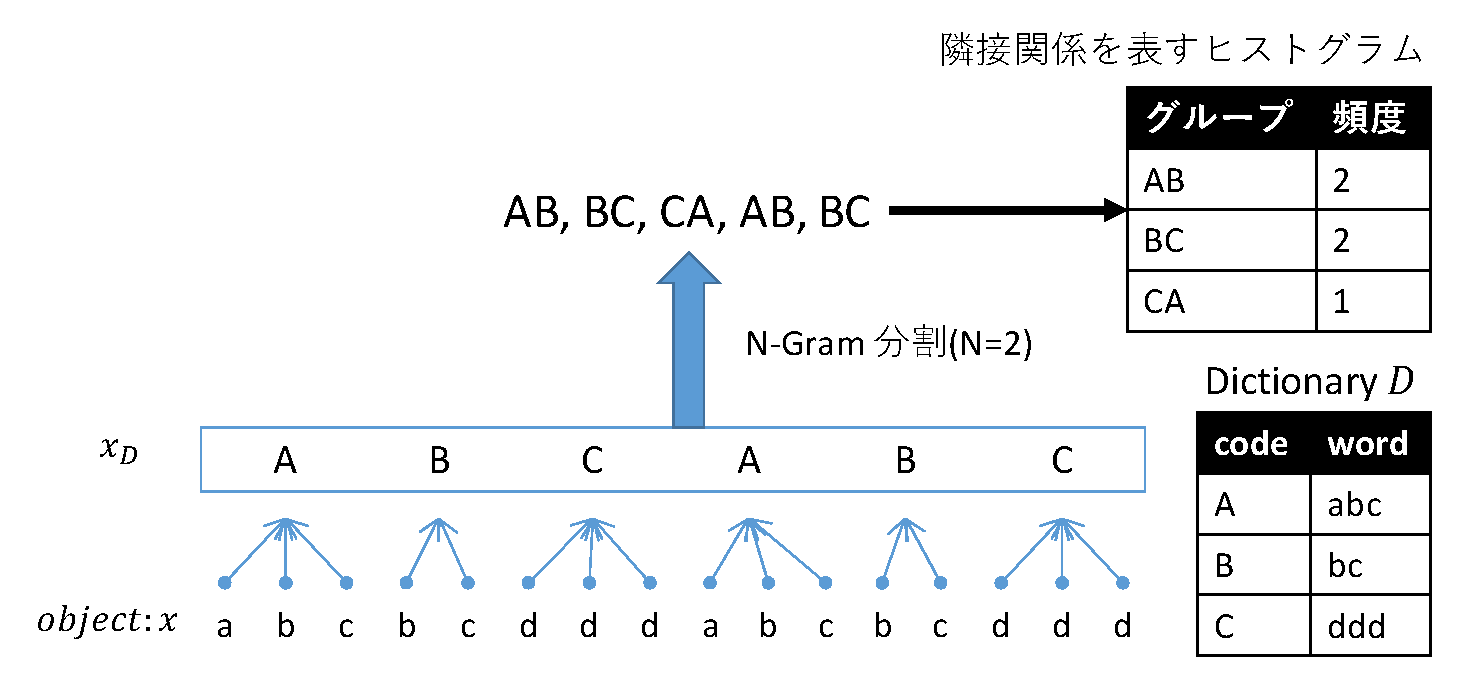
\includegraphics[clip, width=\columnwidth]{image/N-Gram.eps}
\caption{符号列からN-Gramのヒストグラムを作成}
\label{fig:image/N-Gram.eps}
\end{center}
\end{figure}


% section 単語の隣接関係を抽出する単純な手法 (end)

\section{再圧縮による単語の隣接関係の抽出}
\begin{figure}[tb]
\begin{center}
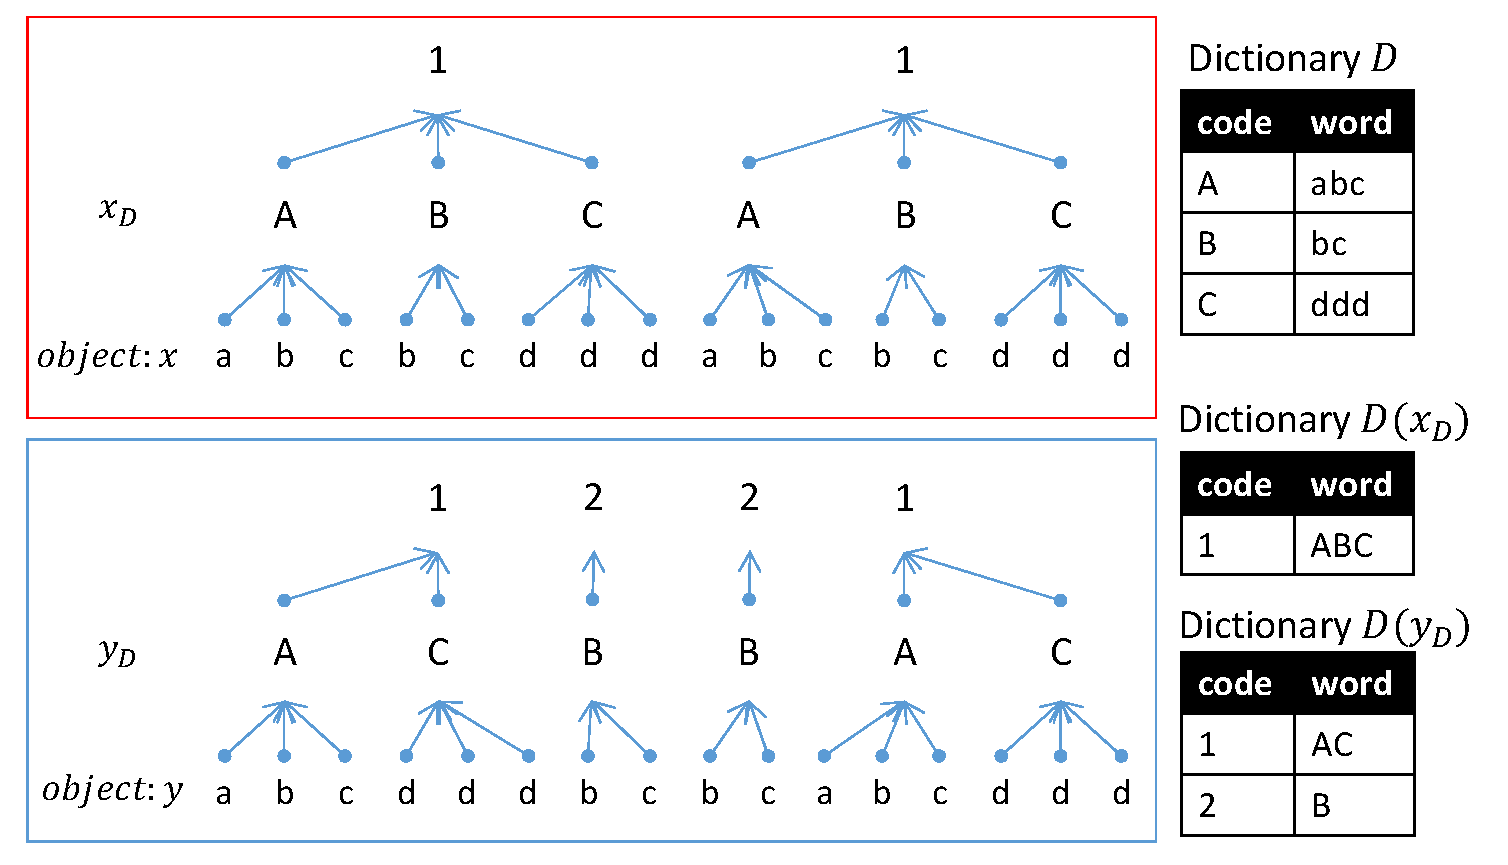
\includegraphics[clip, width=\columnwidth]{image/recompress.eps}
\caption{圧縮後のファイルの再圧縮}
\label{fig:image/recompress.eps}
\end{center}
\end{figure}

本研究では$T$内での単語の隣接関係から定まる新しい特徴量を圧縮後のファイルから抽出する.
具体的には,$T$を辞書$D$で圧縮後のファイル(符号列)を$A^T_D$とすると,$A^T_D$をもう一度再圧縮を行った時の圧縮率を特徴量として採用する.
$A^T_D$の再圧縮では,辞書$D$で圧縮するのではなく,$A^T_D$から構築した辞書で$A^T_D$自身を圧縮する.すなわち,$A^T_D$の自己圧縮率を再圧縮率とする.
再圧縮率の詳しい求め方をAlgorithm\ref{algo:recompress}に示す.
\begin{algorithm}[tb]
\caption{再圧縮率の算出}\label{algo:recompress}
\begin{algorithmic}[1]
\Procedure{CalcRecompressRate}{$A^T_D$}
\Comment{$A^T_D$は1度目の圧縮で出力された符号列}
\State{$Dictionary = 空の辞書$}
\State{$OutputLength = 0$}\Comment{出力長}
\State{$index = 0$}\Comment{辞書番号}
\State{$w = \{\}$}
\For{$i = 1 \, \ldots \, A^T_D.\mathrm{length}$}
\State{$c = A^T_D[i]$}
\State{$wc = w + \{c\}$}\Comment{符号列$w$と符号列$\{c\}$を連結}
\If{$符号列cが辞書に存在しない$}
\State{$Dictionary[\{c\}] = index$}\Comment{初めて出現した符号列$c$を辞書に登録}
\State{$index++$}
\EndIf
\If{$符号列wcが辞書に存在する$}
\State{$w = wc$}
\Else
\State{$Dictionary[wc] = index$}\Comment{符号列$wc$を辞書に登録}
\State{$index++$}
\State{$OutputLength++$}
\State{$w = \{c\}$}
\EndIf
\EndFor
\If{$wが空でない$}
\State{$OutputLength++$}
\EndIf
\State{$RecompressRate = OutputLength / A^T_D.\mathrm{length}$}
\State \textbf{return} $RecompressRate$
\EndProcedure
\end{algorithmic}
\end{algorithm}


再圧縮率が$T$内の単語の隣接関係から定まる特徴であることを例によって示す.
%一度目の圧縮率だけでは分類できないオブジェクトを分類する.
図\ref{fig:image/recompress.eps}は,テキスト$T_1$と$T_2$を再圧縮まで行った時の様子を示す.
最下段が元のテキストであり,真ん中の段が辞書$D$で圧縮後のファイル,最上段が再圧縮後の出力ファイルである.
なお,再圧縮時には自己圧縮を行うため,$T_1$の再圧縮と$T_2$の再圧縮では異なる辞書が用いられている.

辞書$D$で$T_1,T_2$を圧縮後の符号化列はそれぞれ''ABCABC'',''ACBBAC''と異なっている.しかし,圧縮率は
どちらも$\frac{6}{16}=0.375$となって$T_1$と$T_2$は区別できない.これは符号語'A','B','C'の出現回数
が同じであることが理由であり,3.1節で述べたように単語の出現回数のみで決定される圧縮率の限界である.

一方,$T_1$の再圧縮率は$\frac{2}{6}$,$T_2$の再圧縮率は$\frac{4}{6}$と異なる値になり,$T_1$と$T_2$を
区別できる.この違いは$T_1$と$T_2$の単語順序の違いに起因する.例えば,$T_1$の再圧縮率は符号語列
'ABC'が$T_1$内に2回出現した事実を反映する.このように再圧縮率は単語の隣接関係から定まる特徴である.

%xとyの区別がつかない.もう一度圧縮を行うことで,符号列の構造を表した特徴量を抽出する事ができる.
\section{再圧縮率を利用したPRDC}
%\section{圧縮率ベクトル} % (fold)
本節では,前節で提案した再圧縮率をPRDCに組み込んだ手法を提案する.
従来のPRDCでは,テキスト$x$を$N$個の基底辞書集合$\{D_1,D_2,\dots,D_N\}$で圧縮し,その圧縮率を並べた$N$
次元特徴ベクトル(式(\ref{eq:PRDC}))で$x$を表現する.
一方,提案手法では通常の圧縮率と再圧縮率を合わせた特徴ベクトルを構築する.\ref{fig:HOPRDC.eps}

\begin{figure}[tb]
\centering
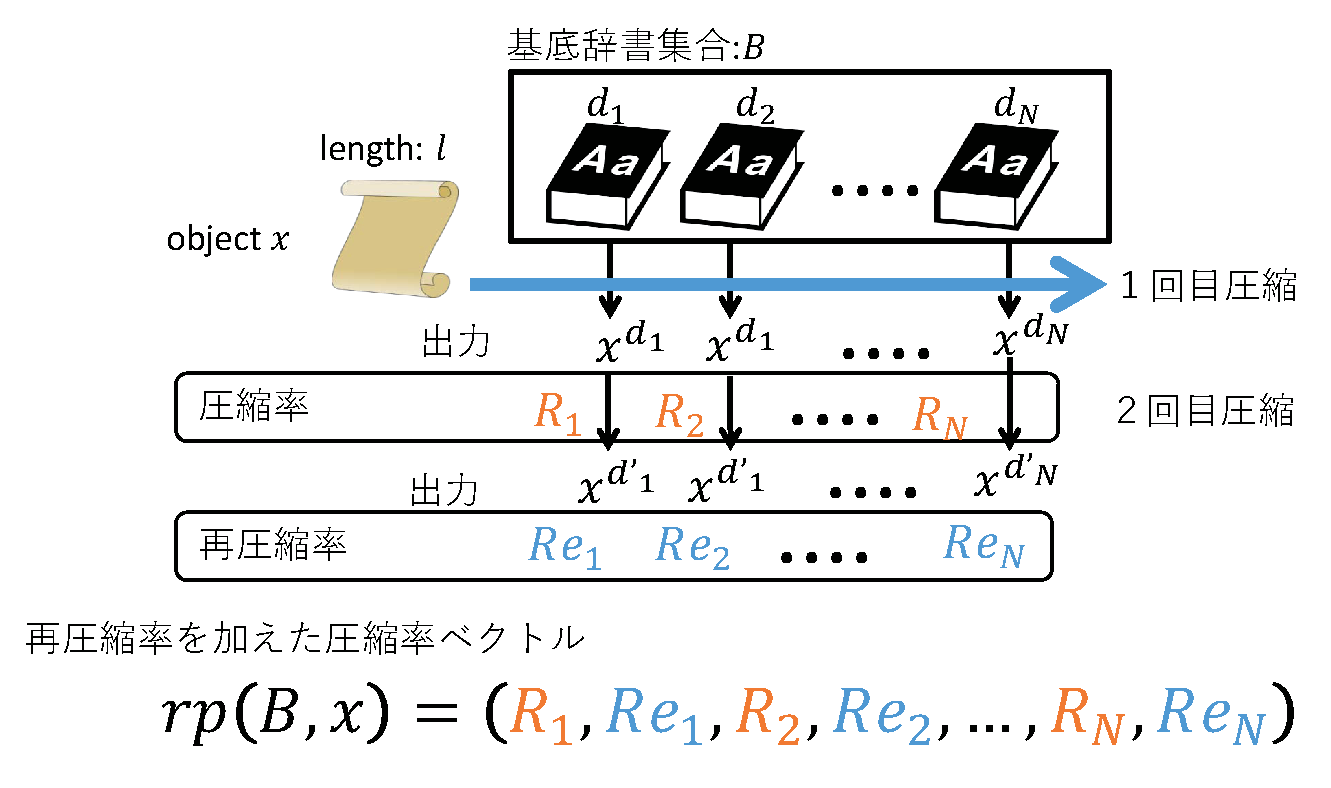
\includegraphics[clip, width=\columnwidth]{image/HOPRDC.eps}
\caption{再圧縮率を加えた圧縮率ベクトルの作成}
\label{fig:HOPRDC.eps}
\end{figure}

基底辞書集合$\{D_1,D_2,\dots,D_N\}$を用いた,オブジェクト$x$に対する再圧縮率を加えた圧縮率ベクトルは
$\boldsymbol{rp}(B,x)$は次のように定義される.
\begin{equation}
\boldsymbol{rp}(B,x) = \biggl(\frac{l'_1}{l}, \frac{l''_1}{l_1'}, \frac{l'_2}{l}, \frac{l''_2}{l'_2}, \dots, \frac{l'_N}{l}, \frac{l''_N}{l'_N} \biggr)
\end{equation}
\begin{itemize}
	\item $l $:入力オブジェクト長
	\item $l'_i$: $x$を$D_i$で圧縮したときの出力長
	\item $l''_i$: $x$を$D_i$で圧縮した符号列を,再圧縮したときの出力長
\end{itemize}
である.1つの基底辞書が2つの次元に対応するので,圧縮率ベクトルの次元数は$2N$になる.この圧縮率ベクトルは
以下の特徴を有する.
\begin{enumerate}
	\item 通常の圧縮率により単語の頻度を考慮する.
	\item 再圧縮率により単語の隣接関係を考慮する.
\end{enumerate}
提案手法では単語の頻度だけでなく単語の隣接関係まで考慮したパターン認識を可能にする.
この性質より,提案手法をHOPRDC (High-Order PRDC, 高階PRDC)と名付ける.

HOPRDCはPRDCと比べて追加のハイパパラメータを必要としておらず,利用の手軽さを失っていない.

%\label{sub:再圧縮率を取り入れたprdc}
\chapter{Weigtbed NMD} % (fold)
本章では,圧縮辞書から特徴抽出を行う手法であるNMDを取り上げ,
圧縮辞書からの新しい特徴抽出によるNMDの改良手法を説明する.
\label{sec:nmdの改良_仮_}
\section{NMDの課題}
NDDやNMDなどの辞書間距離では,辞書を元オブジェクトの要約として用いることで,類似度計算の計算量を削減する.
その一方で,元オブジェクトから情報を捨てることが欠点である.NMDでは各単語の出現回数を考慮し,NDDよりも捨てられる情報を削減した.
しかし,NMDでは辞書に登録された単語長を無視し,全単語は長さによらず均等の重みを持つものとして式(\ref{eq:NMD})の定義
に従って距離計算を実施する.つまり,単語が元のオブジェクトで占めている割合を考慮していない.

図~\ref{fig:image/NMD_Task.eps}は,NMDで使用する多重集合中の単語の割合と,元オブジェクトにおける単語の割合の一例である.オブジェクト$x$は全体で7文字なので,3文字の単語"aaa"がオブジェクト$x$中で占める割合は3/7である.対して,単語"aaa"が多重集合$MS(x)$中で占める割合は,"aaa"の重複度が1なので1/4となる.
このように,NMDのように全単語を均等に取り扱う手法では,元オブジェクトにおいて単語が占める領域の割合と,
各単語が類似度計算に与える影響の割合が乖離する.

\begin{figure}[tb]
\begin{center}
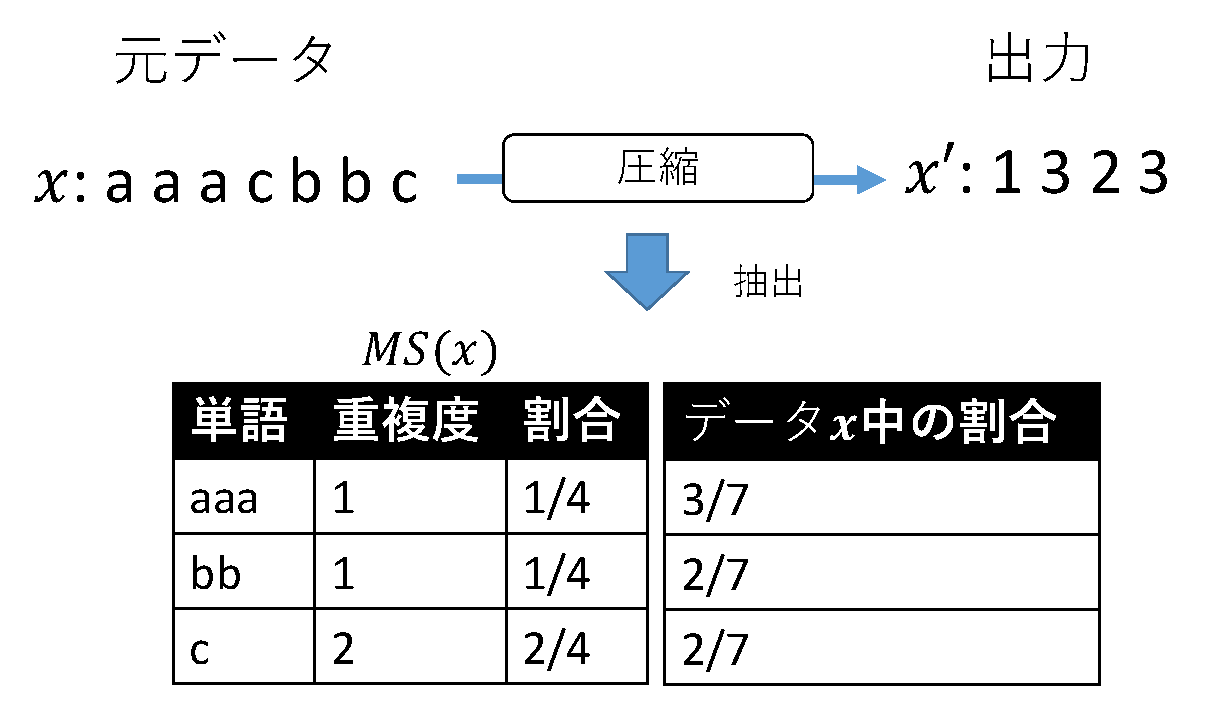
\includegraphics[clip, width=\columnwidth]{image/NMD_Task.eps}
\caption{単語の多重集合中の割合とオブジェクト中の割合}
\label{fig:image/NMD_Task.eps}
\end{center}
\end{figure}

距離計算の際,単語長を無視することがパターン認識に与える影響を考えてみよう.図\ref{fig:created_image.eps}左の画像は,
上半分が単純な領域で,下半分が複雑な領域になっている.このような画像の現実例としては上半分が海で下半分が港湾都市
であるケースが挙げられる.この画像から辞書を作ると,上領域からは長い単語が少数生成され,下領域からは
短い単語が多数生成される(図\ref{fig:created_image.eps}右).この時,全単語を均等に取り扱うということは,
少数の単語を生成する上半分の領域を軽視することを意味する.距離計算においても上半分の領域が軽視されるので,
類似検索の際,上半分が全く同じオブジェクトでも類似していると判定されないという問題が起こり得る.先述した現実例では,
海を含む画像は海を含むという理由では類似していると判定されにくくなるが,これは人間の直観に反する.

% 上記をまとめると,NMDのように全単語を均等に取り扱う手法では,元オブジェクトにおいて単語が占める領域の割合と,
% 各単語が類似度計算に与える影響の割合が乖離する.

%元オブジェクトの単調な領域を軽視することになる.
%
%
%例えば,図\ref{fig:created_image.eps}の左側の画像では,単純な領域が上半分を占めているが,殆どの単語は下半分の複雑な部分から抽出されるため,

\begin{figure}[tb]
\begin{center}
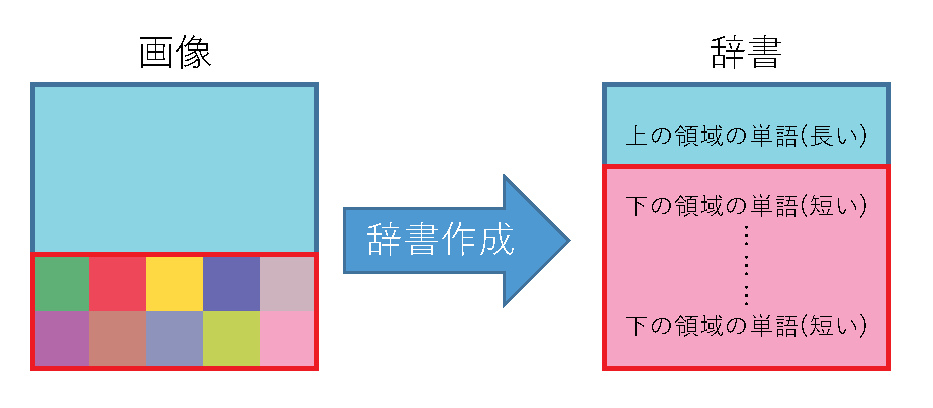
\includegraphics[clip, width=\columnwidth]{image/created_image_1.eps}
\caption{単純な領域と複雑な領域に対する辞書内での単語の割合}
\label{fig:created_image.eps}
\end{center}
\end{figure}
\section{重み付きNMD}
前節で述べた課題に対して,本研究では単語ごとに重みを付けて類似度を計算する
重み付き辞書間距離 WNMD (weigtbed NMD)を提案する.$x,y$間の距離$WNMD(x,y)$は次のように
定義される.
%単語がオブジェクト中で占める長さによらず,類似度計算に与える影響に差がない問題を回避するために,単語ごとに重みをつけることを考える.
%次のような
$$
\frac{G(MS(x) \cup MS(y)) - \min(G(MS(x)) , G(MS(y)))}{\max(G(MS(x)) , G(MS(y)))}
$$
\begin{equation}
G(MS(x)) = \sum_{i=1}^n g(w_i)\times m_i^x
\end{equation}
ここで,$g(w_i)$は単語$w_i$に対する重みである.

% 関数$g$は単語の長さに関して単調増加することが望ましい.
単語に対する重みは,その情報量を表すものが理想だが,正確な情報量は求めることが困難である.
そこで本研究では,単語$w$の重み$g(w)$を,$w$が全て同一文字から構成される場合の最小記述長から定める.

文字列$T=\underbrace{\mbox{aa}\cdots \mbox{a}}_{|w|}$は,$a$が$\sqrt{|w|}$回連続した文字列$A=\underbrace{\mbox{aa}\cdots \mbox{a}}_{\sqrt{|w|}}$を符号語
(モデル)として,$\underbrace{\mbox{AA}\cdots \mbox{A}}_{\sqrt{|w|}}$と表記した時に,
$$記述長=(モデルAの長さ)+(AによるTの符号列長)$$
が最小になる.この時の記述長は$O(\sqrt{|w|})$になることから,$g(|w|)$を式(\ref{eq:weigtbWNMD})とした.ここで,$|w|$は単語$w$の文字数である.
\begin{equation}
\label{eq:weigtbWNMD}
g(w)=\sqrt{|w|}.
\end{equation}

%重みは$log_2(単語の長さ)$とする.
% section nmdの改良_仮_ (end)
\chapter{実験}
2つの提案手法の評価と考察を行うために複数の実験を行った.

\section{HOPRDCにおける圧縮率と再圧縮率の関係} % (fold)
\label{sec:hoprdcにおける圧縮率と再圧縮率の関係}
\begin{figure}[tb]
\begin{center}
\includegraphics[clip, width=\columnwidth]{image/graph-recomp-comp.eps}
\caption{圧縮率と再圧縮率の関係}
\label{fig:image/graph-recomp-comp}
\end{center}
\end{figure}

% \begin{figure}[tb]
% \begin{center}
% 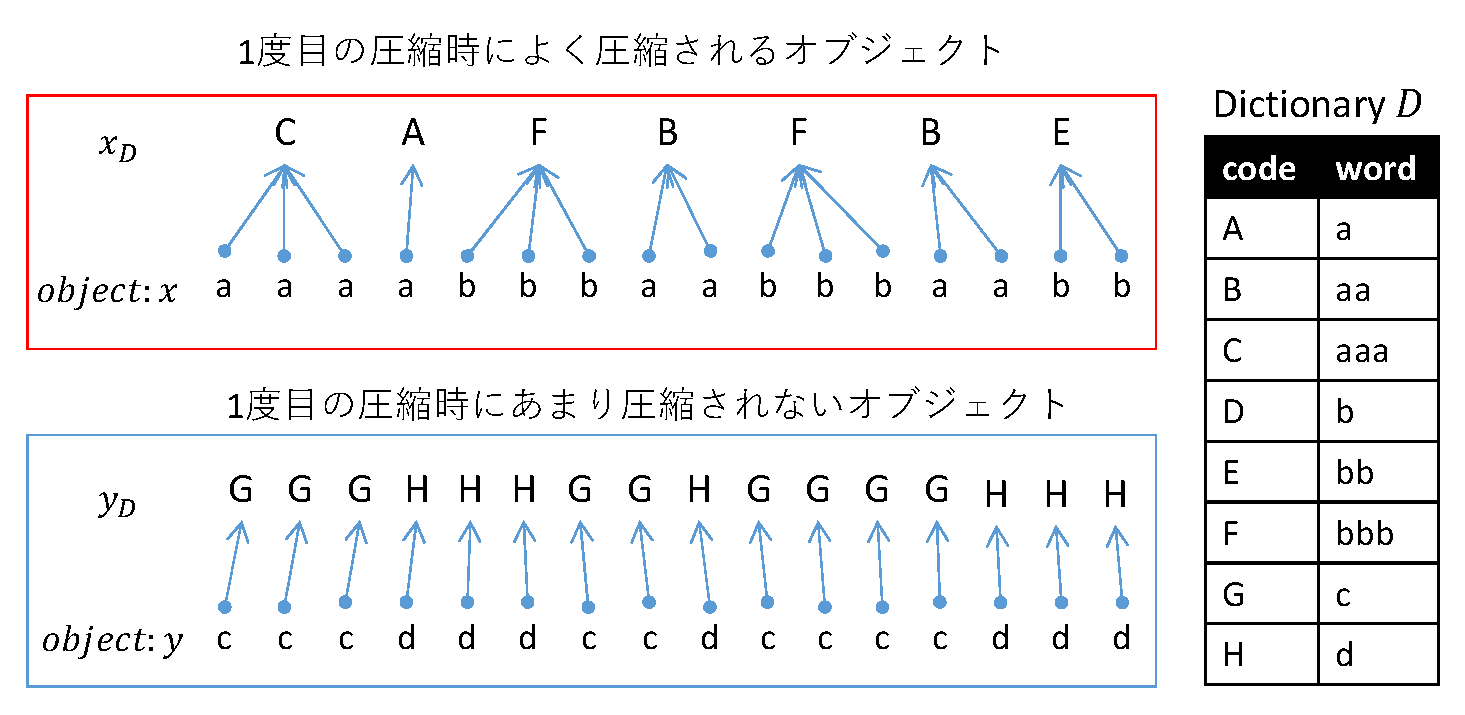
\includegraphics[clip, width=\columnwidth]{image/better-comp-object.eps}
% \caption{よく圧縮されるオブジェクトとあまり圧縮されないオブジェクト}
% \label{fig:image/better-comp-object.eps}
% \end{center}
% \end{figure}


圧縮率と再圧縮率の関係を調査する.
図~\ref{fig:image/graph-recomp-comp}は,Corelデータセットの画像を10個の辞書で圧縮したときの圧縮率と再圧縮率をプロットしたものである.画像ごとの違いを調べるために,11種類の画像をまとめてプロットした.
実験結果より,圧縮率と再圧縮率には負の相関がある,つまり1度目の圧縮でよく圧縮されたデータは,再圧縮時にはあまり圧縮できないことが分かった.
この理由は次のように考えられる.
\begin{itemize}
	\item $l $:入力オブジェクト長
	\item $l'$: $x$を$D$で圧縮したときの出力長
	\item $l''$: $x$を$D$で圧縮した符号列を,再圧縮したときの出力長
\end{itemize}
とするとき,圧縮率は$\frac{l'}{l}$,再圧縮率は$\frac{l''}{l'}$と表される.
ここで$\frac{l''}{l}$も(2回の圧縮を実行する)圧縮アルゴリズムで求めた圧縮率なので,$l''$は$l$が持つ情報量の近似とみなせる.そこで,$l''$を定数とすると,式\ref{eq:comp-recomp-relation}より圧縮率$\frac{l'}{l}$と再圧縮率$\frac{l''}{l'}$は反比例するので,負の相関関係が成り立つ.
\begin{equation}
\label{eq:comp-recomp-relation}
\frac{l'}{l}\times \frac{l''}{l'} = \frac{l''}{l} = 定数
\end{equation}


% 図\ref{fig:image/better-comp-object.eps}
% のように,辞書に登録されていない文字が連続して出現する場合,同じ符号が大量に出力される.その為,出力符号列は単純になり,2度目の圧縮時によく圧縮される.
% 画像ファイルでは,図\ref{fig:image/better-comp-object.eps}のように同じ文字が連続して出現しやすい.よって今回の実験で,圧縮率と再圧縮率に負の相関が見られたと考えられる.

% section hoprdcにおける圧縮率と再圧縮率の関係 (end)

\section{画像分類による性能評価}
\subsection{データセット}
以下の2種類のデータセットを用いて提案手法の画像分類性能を先行研究と比較した.
\begin{itemize}
	\item Corelデータセット~\cite{Corel}
	\item Caltech101 データセット~\cite{Caltech101}
\end{itemize}
\begin{figure}[tb]
\begin{center}
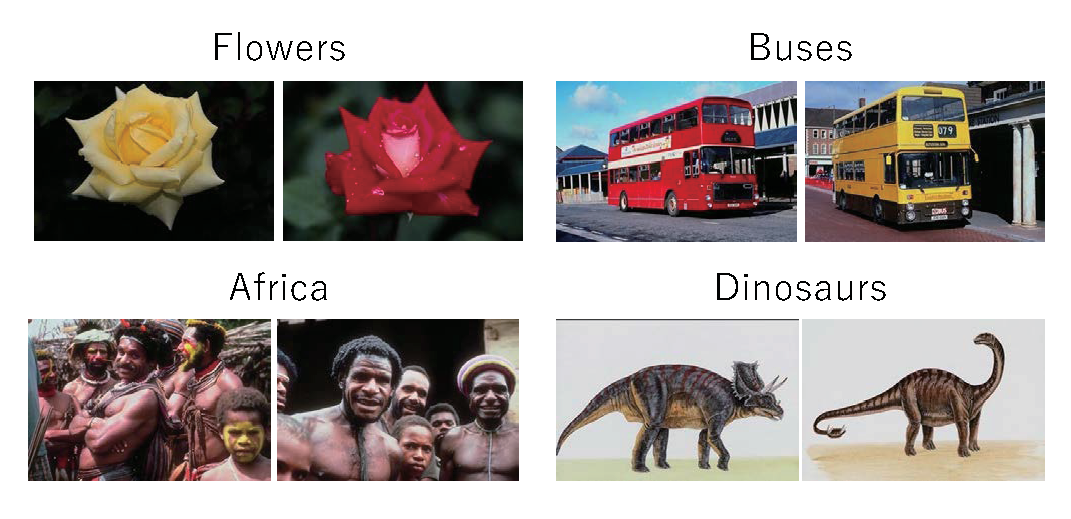
\includegraphics[clip, width=\columnwidth]{image/dataset.eps}
\caption{Corelデータセットの一部}
\label{fig:image/dataset.eps}
\end{center}
\end{figure}
Corelデータセットは先行研究~\cite{NMD}で実験に用いられたものと同じである.このデータセットはCorel image repository~\cite{Corel}の画像からなり,[256×384]か[384×256]の画像が1000枚,100枚づつ10個のクラスに分けられている.その一部を図\ref{fig:image/dataset.eps}に示す.
Caltech101データセットは画像分類においてよく用いられるデータセットである.このデータセットは9146枚の画像からなり,101個のカテゴリに分けられている.これらのカテゴリには少ないもので30枚,多いもので800枚の画像が含まれている.
\subsection{画像のテキスト化}
画像は2次元データなので,圧縮パターン認識に適用するには,1次元のテキストに変換する必要がある.
そこで,先行研究~\cite{NMD}と同様に,各画素のrgb値をそれぞれ5段階に量子化して,125種類の文字で表現し,これらを水平スキャンで連結してテキストに変換した.

\subsection{HOPRDCの評価結果}
PRDCとHOPRDCを比較するためCorelクラス分類実験を行う.
データセットからランダムに10枚画像を選択し,各画像から1つずつ,合計10個の基底辞書を作成する.その後ランダムに890枚選択した画像を学習画像とし,残りの画像100枚をクエリとして用いる.
クエリ画像の分類は次の手順で行う.
\begin{enumerate}
	\item クエリ画像を圧縮率ベクトルに変換する
	\item クエリ画像をk-NN法でクラス分類する.クエリと最近の$k$枚の学習画像を求め,その中で枚数が最も多いクラスに分類する.
\end{enumerate}
今回の実験では$k$=5とした.
判別率$r$は次のように計算する.
\begin{equation}
r=\frac{正しく分類されたテスト画像数}{テスト画像数}
\end{equation}

% 各クラス$c$の判別率$r_c$は次のように計算する.
% \begin{equation}
% r_c=\frac{正しく分類されたクラスcのデータ数}{テスト画像中のクラスcのデータ数}
% \end{equation}

\begin{figure}[tb]
\begin{center}
\includegraphics[clip, width=\columnwidth]{image/PRDCvsProposed.eps}
\caption{クラス毎の判別率(クエリの数は100枚,基底辞書の個数は10個,試行回数は300回)}
\label{fig:PRDCvsProposed.eps}
\end{center}
\end{figure}
\begin{table}
\caption{全画像に対する判別率}
\label{tab:Average_PRDCvsProposed}
\begin{center}
\begin{tabular}{|l||l|}
\hline
PRDC   & 0.6393 \\
\hline
HOPRDC & 0.6798 \\
\hline
\end{tabular}
\end{center}
\end{table}
本実験では基底辞書をランダムに選択するため,300回の試行を行いその平均値を報告する.

表\ref{tab:Average_PRDCvsProposed}は前テスト画像に対する判別率である.HOPRDCはPRDCに比べて4\%程度判別率が向上した.
図\ref{fig:PRDCvsProposed.eps}はクラスごとの判別率である.
提案手法では,BusクラスやFlowerクラスにおいてPRDCを大きく上回った.この2つのクラスのインスタンスには,同じ形で色が違うものが含まれる.PRDCでは,単語の頻度のみを考慮しているため,オブジェクトの色に認識結果が大きく左右される.一方,提案手法では,再圧縮率により単語の隣接関係を考慮するため,オブジェクトの形も認識結果に影響を与える.

図\ref{fig:PRDC_HOPRDC_retrival.eps}はPRDCとHOPRDCで作成したベクトルを用いて,類似画像検索を行った結果の一例である.PRDCでは,赤い色のピクセルの割合がクエリ画像と似ているものが上位に来ている.HOPRDCでは,赤いピクセルの割合が似ているだけではなく,赤いピクセルの形が似ているものが上位に来ている.
再圧縮率で単語の順序関係を考慮したことで,オブジェクトの形が似ているものが抽出されやすくなったことが確認できる.

\begin{figure}[tb]
\centering
\includegraphics[clip, width=\columnwidth]{image/PRDC_HOPRDC_retrival.eps}
\caption{PRDCとHOPRDCの類似画像検索結果例}
\label{fig:PRDC_HOPRDC_retrival.eps}
\end{figure}


\subsection{WNMDの評価結果}
提案手法であるWNMDと,現在辞書間距離の中で最も精度が高いNMDを比較するため,2つのデータセットを使い類似画像検索を行う.
Corelデータセットを用いた実験では,データベースに1000枚の画像全てを登録する.クエリはこの中の1枚を使用する.クエリとデータベースの全画像間で類似度計算を行い,類似度が高い上位100枚の画像を検索結果とする.
クエリ画像$Q$に対する検索結果は式(\ref{equ:Precision_Corel})に示す適合率で評価する.分母の100は検索結果の画像数であるが,1クラスあたりの画像数とも一致する.
\begin{equation}
P(Q) = \frac{N_r}{100}
\label{equ:Precision_Corel}
\end{equation}
ここで$N_r$は検索結果の中でクエリ画像Qと同じクラスの画像の枚数である.
全ての画像をクエリとして使い,1000回類似画像検索を行った平均適合率によりアルゴリズムの性能を評価する.

Caltech101データセットを用いた実験では,データベースに9146枚の画像全てを登録する.クエリはこの中の1枚を使用する.クエリとデータベースの全画像間で類似度計算を行い,類似度が高い上位30枚の画像を検索結果とする.
クエリ画像$Q$に対する検索結果は式(\ref{equ:Precision_Caltech})に示す適合率で評価する.分母の30は検索結果の画像数である.
\begin{equation}
P(Q) = \frac{N_r}{30}
\label{equ:Precision_Caltech}
\end{equation}

\begin{figure}[tb]
\begin{center}
\includegraphics[clip, width=\columnwidth]{image/NMDvsProposed.eps}
\caption{NMDと提案手法の平均適合率の比較(クエリはデータセット中の全ての画像)}
\label{fig:NMDvsProposed.eps}
\end{center}
\end{figure}
\begin{table}
\caption{全画像に対する平均適合率}
\label{tab:Average_NMDvsProposed}
\begin{center}
\begin{tabular}{|l||l|l|}
\hline
&Corel&Caltech101 \\
\hline
NMD  & 0.509 & 0.312\\
\hline
WNMD & 0.530 & 0.337\\
\hline
\end{tabular}
\end{center}
\end{table}

% Table generated by Excel2LaTeX from sheet 'Sheet1'
\begin{table}[htbp]
\centering
\caption{重みの評価}
\begin{tabular}{|l|r|}
\hline
\textbf{重み} &
\multicolumn{1}{l|}{\textbf{適合率}}
\bigstrut\\
\hline
$\log_2 (|w|+1)$ &
0.524
\bigstrut\\
\hline
$\sqrt{|w|}$ &
0.53
\bigstrut\\
\hline
$|w|$ &
0.519
\bigstrut\\
\hline
    \end{tabular}%
  \label{tab:NMD_weight_compare}%
\end{table}%

表\ref{tab:Average_NMDvsProposed}に全画像に対する平均適合率を示す.
CorelデータセットではWNMDはNMDと比べて1.6\%程度適合率が向上した.
Caltech101データセットでは約2.5\%適合率が向上した.

WNMDがどのような画像に対して有効に働いているかを知るために,Corelデータセットに対しての結果を詳しく調べる.
図\ref{fig:NMDvsProposed.eps}にNMDとWNMDのクラスごとの平均適合率を示す.
提案手法ではAfricaクラスや,DinosaursクラスにおいてNMDを大きく上回った.
この2つのクラスでは,同色で単純な領域が広い面積を占める画像が多い.
Africaクラスには人物を映した画像が多く,肌色の単純な領域が大きい.
Dinosoursクラスでは,背景や恐竜の肌が少ない色で表現されており,単純である.
NMDでは単純領域の特徴を軽視するのに対し,WNMDでは,単語に長さに応じた重みをつけることで,これらのクラスで重要な特徴となる単純な領域を軽視せずに類似計算を行うことができ,精度が向上した.
\subsection{重み付け関数$g(w)$の評価} % (fold)
\label{sub:重み付け関数}
長さに対する重みが適切かどうかの実験を行った.
単語$w$の長さを$|w|$としたとき,$\sqrt{|w|}$,$|w|$,$\log_2 (|w|+1)$の3種類の重みを比較した.
ここで,$log_2(|w|+1)$は,全ての文字が同じ単語の情報量,$|w|$は全ての文字が違う単語の情報量である.
比較はCorelデータセットで式\ref{equ:Precision_Corel}を用いて行った.結果は表~\ref{tab:NMD_weight_compare}に示す.実験より,$\sqrt{|w|}$が最も高い精度であることがわかる.

% subsection 重み付け関数 (end)

\section{時系列データ分類による性能評価} % (fold)
\label{sub:時系列データ分類による性能評価}
提案手法が画像以外のデータセットに対して有効かどうかを調べるために,様々な種類の時系列データに対して分類実験を行った.
\subsection{UCR Time Series Classification Archive} % (fold)
\label{sub:UCR Time Series Classification Archive}
UCR Time Series Classification Archive~\cite{UCRArchive}(以下 UCR Archive)は,様々な種類の時系列データを集めたデータセット集である.
現在このデータセット集には全部で85種類のデータセットが用意されており,全てが同じフォーマットで記述されている.そのため,手軽に多種多様なデータに対しての分類精度を比較することができる.
% subsection UCR Time Series Classification Archive (end)
\subsection{データのテキスト化} % (fold)
\label{sub:データのテキスト化}
圧縮パターン認識に適用するために,時系列データを1次元のテキストに変換する.
全てのTESTデータとTRAINデータの値を125,60,30,15レベルに量子化し,文字に置き換えた.

\begin{figure}[tb]
\begin{center}
\includegraphics[clip, width=\columnwidth]{image/DataEncode.eps}
\end{center}
\caption{データのテキスト化}
\label{fig:DataEncode.eps}
\end{figure}
% subsection subsection_name (end)

\subsection{クラス分類実験} % (fold)
\label{sub:クラス分類実験}
クラス分類実験の方法について説明する.
UCRArchiveのデータセットはそれぞれTESTデータとTRAINデータに予め分けられている.
実験では,TRAINデータを用いて,TESTデータを1-NNでクラス分類したときの分類精度を評価する.

PRDC・HOPRDCを用いた分類実験では,TRAINデータの各クラスから2つずつデータを選び,それを基底辞書として用いる.(例えば,3クラス分類の場合,基底辞書は全部で6つ,PRDCでは6次元,HOPRDCでは12次元のベクトルが作成される.)
TESTデータから作成した圧縮率ベクトルとTRAINデータの圧縮率ベクトルとのユークリッド距離を用いて1-NN分類を行う.
このとき,基底辞書の選択により分類精度が変動するので,100回の分類実験を行いその平均を評価する.

NMD・WNMDを用いた分類実験では,TESTデータとTRAINデータから辞書を作成し,辞書間距離NMD・WNMDを用いて1-NN分類を行う.
% subsection クラス分類実験 (end)
\subsection{実験結果} % (fold)
\label{sub:実験結果}
表\ref{tab:HOPRDC_UP_AND_DOWN},表\ref{tab:WNMD_UP_AND_DOWN}に実験の結果,精度が向上したデータセットの個数と,変化しなかった個数,低下した個数をまとめた.結果の詳細は付録に掲載する.
実験より,HOPRDC,WNMDは多くのデータセットに対し,有効であるという結果が得られた.しかし,精度が低下してしまったデータセットも存在するので,どのようなデータについて有効なのかを詳しく考察する.

HOPRDCでは図\ref{fig:image/HOPRDC_up_down.eps}左のようなデータセットでは精度が低下した.このデータセットは全てのデータの大まかな構造が同じなので,クラス分類においては細かい部分の違いが大きく影響する.HOPRDCではデータの大まかな構造を重視するため,精度が低下したと考えられる.このようなデータセットは,データの記述に数値の微分を用いると,データの特徴を表現でき,うまく分類できるようになると考えられる.
逆に,図\ref{fig:image/HOPRDC_up_down.eps}右のような,カテゴリごとにデータの大まかな形が異なるデータセットでは,大きく精度が向上した.また,データを15分割したとき,HOPRDCは先行研究と比べて大きな向上が見られなかった.15分割では多くのデータが同じような形で表現されるので,HOPRDCで用いている単語の隣接関係の情報があまり役に立たないことが原因と考えられる.

WNMDでは,図~\ref{fig:image/WNMD_up_down.eps}左側のような,数値の高さのみが分類に重要なデータセットでは精度が低下した.逆に,分類にデータの数値が出現する位置が重要なデータで精度が向上した.
また,125分割,60分割のとき,WNMDは先行研究と比べ同程度の結果となったが,これはデータから作成された辞書中に長い単語が殆ど出現していないことが要因である.

% Table generated by Excel2LaTeX from sheet 'Sheet1'
\begin{table}[htbp]
\centering
\caption{HOPRDCでPRDCよりも精度が向上(低下)したデータセットの数}
\begin{tabular}{|l|r|r|r|r|}
\cline{2-5}    \multicolumn{1}{r|}{} &
\multicolumn{1}{c|}{125分割} &
\multicolumn{1}{c|}{60分割} &
\multicolumn{1}{c|}{30分割} &
\multicolumn{1}{c|}{15分割}
\bigstrut\\
\hline
向上 &
52 &
51 &
51 &
40
\bigstrut\\
\hline
変化なし &
0 &
2 &
2 &
2
\bigstrut\\
\hline
低下 &
26 &
25 &
25 &
36
\bigstrut\\
\hline
    \end{tabular}%
  \label{tab:HOPRDC_UP_AND_DOWN}%
\end{table}%

% Table generated by Excel2LaTeX from sheet 'Sheet1'
\begin{table}[htbp]
\centering
\caption{WNMDでNMDよりも精度が向上(低下)したデータセットの数}
\begin{tabular}{|l|r|r|r|r|}
\cline{2-5}    \multicolumn{1}{r|}{} &
\multicolumn{1}{c|}{125分割} &
\multicolumn{1}{c|}{60分割} &
\multicolumn{1}{c|}{30分割} &
\multicolumn{1}{c|}{15分割}
\bigstrut\\
\hline
向上 &
41 &
41 &
49 &
47
\bigstrut\\
\hline
変化なし &
9 &
4 &
5 &
7
\bigstrut\\
\hline
低下 &
35 &
40 &
31 &
31
\bigstrut\\
\hline
    \end{tabular}%
  \label{tab:WNMD_UP_AND_DOWN}%
\end{table}%


% subsection 実験結果 (end)
% % Table generated by Excel2LaTeX from sheet 'split30 k=1'
\begin{longtable}[c]{|l||r||r|r||r|r|}
\caption{データを30分割したときの精度比較}
\\
\hline
\textbf{データセット名} &
\multicolumn{1}{l||}{\textbf{Euclidean}} &
\multicolumn{1}{l|}{\textbf{PRDC}} &
\multicolumn{1}{l||}{\textbf{HOPRDC}} &
\multicolumn{1}{l|}{\textbf{NMD}} &
\multicolumn{1}{l|}{\textbf{WNMD}}
\bigstrut\\
\hline
\endhead
\rowcolor[rgb]{ .851,  .851,  .851} 50words &
0.631 &
&
&
0.321 &
\cellcolor[rgb]{ .973,  .796,  .678} \textbf{0.327}
\bigstrut[t]\\
Adiac &
0.611 &
\cellcolor[rgb]{ .973,  .796,  .678} \textbf{0.459} &
0.39 &
0.317 &
\cellcolor[rgb]{ .973,  .796,  .678} \textbf{0.345}
\\
\rowcolor[rgb]{ .851,  .851,  .851} ArrowHead &
0.8 &
\cellcolor[rgb]{ .973,  .796,  .678} \textbf{0.597} &
0.582 &
\cellcolor[rgb]{ .973,  .796,  .678} \textbf{0.651} &
0.629
\\
Beef &
0.667 &
\cellcolor[rgb]{ .973,  .796,  .678} \textbf{0.45} &
0.443 &
0.567 &
\cellcolor[rgb]{ .973,  .796,  .678} \textbf{0.6}
\\
\rowcolor[rgb]{ .851,  .851,  .851} BeetleFly &
0.75 &
\cellcolor[rgb]{ .973,  .796,  .678} \textbf{0.735} &
0.66 &
0.8 &
\cellcolor[rgb]{ .973,  .796,  .678} \textbf{0.9}
\\
BirdChicken &
0.55 &
0.745 &
\cellcolor[rgb]{ .973,  .796,  .678} \textbf{0.765} &
0.8 &
\cellcolor[rgb]{ .973,  .796,  .678} \textbf{0.85}
\\
\rowcolor[rgb]{ .851,  .851,  .851} Car &
0.733 &
0.41 &
\cellcolor[rgb]{ .973,  .796,  .678} \textbf{0.43} &
0.583 &
\cellcolor[rgb]{ .973,  .796,  .678} \textbf{0.667}
\\
CBF &
0.852 &
\cellcolor[rgb]{ .973,  .796,  .678} \textbf{0.641} &
0.639 &
\cellcolor[rgb]{ .973,  .796,  .678} \textbf{0.661} &
0.659
\\
\rowcolor[rgb]{ .851,  .851,  .851} ChlorineConcentration &
0.65 &
0.499 &
\cellcolor[rgb]{ .973,  .796,  .678} \textbf{0.504} &
\cellcolor[rgb]{ .973,  .796,  .678} \textbf{0.547} &
0.541
\\
CinC\_ECG\_torso &
0.897 &
0.446 &
\cellcolor[rgb]{ .973,  .796,  .678} \textbf{0.544} &
\cellcolor[rgb]{ .973,  .796,  .678} \textbf{0.605} &
0.594
\\
\rowcolor[rgb]{ .851,  .851,  .851} Coffee &
1 &
0.618 &
\cellcolor[rgb]{ .973,  .796,  .678} \textbf{0.629} &
\cellcolor[rgb]{ .973,  .796,  .678} \textbf{0.821} &
0.786
\\
Computers &
0.576 &
0.62 &
\cellcolor[rgb]{ .973,  .796,  .678} \textbf{0.629} &
\cellcolor[rgb]{ .973,  .796,  .678} \textbf{0.612} &
0.58
\\
\rowcolor[rgb]{ .851,  .851,  .851} Cricket\_X &
0.577 &
\cellcolor[rgb]{ .973,  .796,  .678} \textbf{0.409} &
0.403 &
0.426 &
\cellcolor[rgb]{ .973,  .796,  .678} \textbf{0.436}
\\
Cricket\_Y &
0.567 &
\cellcolor[rgb]{ .973,  .796,  .678} \textbf{0.359} &
0.353 &
0.405 &
\cellcolor[rgb]{ .973,  .796,  .678} \textbf{0.436}
\\
\rowcolor[rgb]{ .851,  .851,  .851} Cricket\_Z &
0.587 &
\cellcolor[rgb]{ .973,  .796,  .678} \textbf{0.375} &
0.373 &
0.41 &
\cellcolor[rgb]{ .973,  .796,  .678} \textbf{0.413}
\\
DiatomSizeReduction &
0.935 &
&
&
0.846 &
\cellcolor[rgb]{ .973,  .796,  .678} \textbf{0.859}
\\
\rowcolor[rgb]{ .851,  .851,  .851} DistalPhalanxOutlineAgeGroup &
0.783 &
0.727 &
\cellcolor[rgb]{ .973,  .796,  .678} \textbf{0.75} &
\cellcolor[rgb]{ .973,  .796,  .678} \textbf{0.728} &
0.723
\\
DistalPhalanxOutlineCorrect &
0.752 &
0.661 &
\cellcolor[rgb]{ .973,  .796,  .678} \textbf{0.664} &
0.695 &
\cellcolor[rgb]{ .973,  .796,  .678} \textbf{0.698}
\\
\rowcolor[rgb]{ .851,  .851,  .851} DistalPhalanxTW &
0.728 &
0.691 &
\cellcolor[rgb]{ .973,  .796,  .678} \textbf{0.692} &
0.688 &
\cellcolor[rgb]{ .973,  .796,  .678} \textbf{0.698}
\\
Earthquakes &
0.674 &
0.73 &
\cellcolor[rgb]{ .973,  .796,  .678} \textbf{0.731} &
0.724 &
\cellcolor[rgb]{ .973,  .796,  .678} \textbf{0.733}
\\
\rowcolor[rgb]{ .851,  .851,  .851} ECG200 &
0.88 &
0.6 &
\cellcolor[rgb]{ .973,  .796,  .678} \textbf{0.652} &
\cellcolor[rgb]{ .973,  .796,  .678} \textbf{0.7} &
0.69
\\
ECG5000 &
0.925 &
&
&
0.899 &
\cellcolor[rgb]{ .973,  .796,  .678} \textbf{0.902}
\\
\rowcolor[rgb]{ .851,  .851,  .851} ECGFiveDays &
0.797 &
0.632 &
\cellcolor[rgb]{ .973,  .796,  .678} \textbf{0.674} &
0.741 &
\cellcolor[rgb]{ .973,  .796,  .678} \textbf{0.746}
\\
ElectricDevices &
0.549 &
0.561 &
\cellcolor[rgb]{ .973,  .796,  .678} \textbf{0.607} &
0.631 &
\cellcolor[rgb]{ .973,  .796,  .678} \textbf{0.633}
\\
\rowcolor[rgb]{ .851,  .851,  .851} FaceAll &
0.714 &
\cellcolor[rgb]{ .973,  .796,  .678} \textbf{0.296} &
0.294 &
0.325 &
\cellcolor[rgb]{ .973,  .796,  .678} \textbf{0.37}
\\
FaceFour &
0.784 &
0.51 &
\cellcolor[rgb]{ .973,  .796,  .678} \textbf{0.52} &
\cellcolor[rgb]{ .973,  .796,  .678} \textbf{0.636} &
0.625
\\
\rowcolor[rgb]{ .851,  .851,  .851} FacesUCR &
0.769 &
\cellcolor[rgb]{ .973,  .796,  .678} \textbf{0.382} &
0.374 &
0.411 &
\cellcolor[rgb]{ .973,  .796,  .678} \textbf{0.428}
\\
FISH &
0.783 &
0.237 &
0.237 &
\cellcolor[rgb]{ .973,  .796,  .678} \textbf{0.44} &
0.429
\\
\rowcolor[rgb]{ .851,  .851,  .851} FordA &
0.659 &
0.629 &
\cellcolor[rgb]{ .973,  .796,  .678} \textbf{0.653} &
0.61 &
\cellcolor[rgb]{ .973,  .796,  .678} \textbf{0.618}
\\
FordB &
0.558 &
0.615 &
\cellcolor[rgb]{ .973,  .796,  .678} \textbf{0.635} &
0.534 &
\cellcolor[rgb]{ .973,  .796,  .678} \textbf{0.561}
\\
\rowcolor[rgb]{ .851,  .851,  .851} Gun\_Point &
0.913 &
0.788 &
\cellcolor[rgb]{ .973,  .796,  .678} \textbf{0.793} &
\cellcolor[rgb]{ .973,  .796,  .678} \textbf{0.867} &
0.86
\\
Ham &
0.6 &
0.481 &
\cellcolor[rgb]{ .973,  .796,  .678} \textbf{0.485} &
0.457 &
\cellcolor[rgb]{ .973,  .796,  .678} \textbf{0.524}
\\
\rowcolor[rgb]{ .851,  .851,  .851} HandOutlines &
0.801 &
\cellcolor[rgb]{ .973,  .796,  .678} \textbf{0.645} &
0.628 &
0.666 &
\cellcolor[rgb]{ .973,  .796,  .678} \textbf{0.682}
\\
Haptics &
0.37 &
0.238 &
\cellcolor[rgb]{ .973,  .796,  .678} \textbf{0.255} &
\cellcolor[rgb]{ .973,  .796,  .678} \textbf{0.266} &
0.227
\\
\rowcolor[rgb]{ .851,  .851,  .851} Herring &
0.516 &
\cellcolor[rgb]{ .973,  .796,  .678} \textbf{0.563} &
0.497 &
0.594 &
0.594
\\
InlineSkate &
0.342 &
\cellcolor[rgb]{ .973,  .796,  .678} \textbf{0.277} &
0.259 &
0.351 &
\cellcolor[rgb]{ .973,  .796,  .678} \textbf{0.356}
\\
\rowcolor[rgb]{ .851,  .851,  .851} InsectWingbeatSound &
0.562 &
0.159 &
\cellcolor[rgb]{ .973,  .796,  .678} \textbf{0.169} &
0.178 &
\cellcolor[rgb]{ .973,  .796,  .678} \textbf{0.183}
\\
ItalyPowerDemand &
0.955 &
\cellcolor[rgb]{ .973,  .796,  .678} \textbf{0.615} &
0.613 &
0.729 &
\cellcolor[rgb]{ .973,  .796,  .678} \textbf{0.736}
\\
\rowcolor[rgb]{ .851,  .851,  .851} LargeKitchenAppliances &
0.493 &
\cellcolor[rgb]{ .973,  .796,  .678} \textbf{0.661} &
0.6 &
\cellcolor[rgb]{ .973,  .796,  .678} \textbf{0.739} &
0.699
\\
Lighting2 &
0.754 &
\cellcolor[rgb]{ .973,  .796,  .678} \textbf{0.693} &
0.69 &
0.656 &
0.656
\\
\rowcolor[rgb]{ .851,  .851,  .851} Lighting7 &
0.575 &
0.484 &
\cellcolor[rgb]{ .973,  .796,  .678} \textbf{0.512} &
0.589 &
\cellcolor[rgb]{ .973,  .796,  .678} \textbf{0.616}
\\
MALLAT &
0.914 &
&
&
0.831 &
\cellcolor[rgb]{ .973,  .796,  .678} \textbf{0.839}
\\
\rowcolor[rgb]{ .851,  .851,  .851} Meat &
0.933 &
0.557 &
\cellcolor[rgb]{ .973,  .796,  .678} \textbf{0.6} &
0.883 &
0.883
\\
MedicalImages &
0.684 &
0.485 &
\cellcolor[rgb]{ .973,  .796,  .678} \textbf{0.494} &
\cellcolor[rgb]{ .973,  .796,  .678} \textbf{0.568} &
0.551
\\
\rowcolor[rgb]{ .851,  .851,  .851} MiddlePhalanxOutlineAgeGroup &
0.74 &
0.72 &
\cellcolor[rgb]{ .973,  .796,  .678} \textbf{0.722} &
\cellcolor[rgb]{ .973,  .796,  .678} \textbf{0.735} &
0.715
\\
MiddlePhalanxOutlineCorrect &
0.753 &
0.53 &
0.53 &
0.603 &
\cellcolor[rgb]{ .973,  .796,  .678} \textbf{0.61}
\\
\rowcolor[rgb]{ .851,  .851,  .851} MiddlePhalanxTW &
0.561 &
0.551 &
\cellcolor[rgb]{ .973,  .796,  .678} \textbf{0.559} &
\cellcolor[rgb]{ .973,  .796,  .678} \textbf{0.579} &
0.574
\\
MoteStrain &
0.879 &
0.653 &
\cellcolor[rgb]{ .973,  .796,  .678} \textbf{0.671} &
\cellcolor[rgb]{ .973,  .796,  .678} \textbf{0.74} &
0.736
\\
\rowcolor[rgb]{ .851,  .851,  .851} NonInvasiveFatalECG\_Thorax1 &
0.829 &
\cellcolor[rgb]{ .973,  .796,  .678} \textbf{0.518} &
0.465 &
0.518 &
0.518
\\
NonInvasiveFatalECG\_Thorax2 &
0.88 &
\cellcolor[rgb]{ .973,  .796,  .678} \textbf{0.567} &
0.533 &
\cellcolor[rgb]{ .973,  .796,  .678} \textbf{0.619} &
0.608
\\
\rowcolor[rgb]{ .851,  .851,  .851} OliveOil &
0.867 &
0.567 &
\cellcolor[rgb]{ .973,  .796,  .678} \textbf{0.583} &
\cellcolor[rgb]{ .973,  .796,  .678} \textbf{0.833} &
0.8
\\
OSULeaf &
0.521 &
0.464 &
\cellcolor[rgb]{ .973,  .796,  .678} \textbf{0.465} &
0.537 &
\cellcolor[rgb]{ .973,  .796,  .678} \textbf{0.541}
\\
\rowcolor[rgb]{ .851,  .851,  .851} PhalangesOutlinesCorrect &
0.761 &
\cellcolor[rgb]{ .973,  .796,  .678} \textbf{0.605} &
0.6 &
0.652 &
\cellcolor[rgb]{ .973,  .796,  .678} \textbf{0.662}
\\
Phoneme &
0.109 &
&
&
0.197 &
\cellcolor[rgb]{ .973,  .796,  .678} \textbf{0.206}
\\
\rowcolor[rgb]{ .851,  .851,  .851} Plane &
0.962 &
\cellcolor[rgb]{ .973,  .796,  .678} \textbf{0.901} &
0.889 &
0.962 &
0.962
\\
ProximalPhalanxOutlineAgeGroup &
0.785 &
\cellcolor[rgb]{ .973,  .796,  .678} \textbf{0.747} &
0.735 &
\cellcolor[rgb]{ .973,  .796,  .678} \textbf{0.829} &
0.805
\\
\rowcolor[rgb]{ .851,  .851,  .851} ProximalPhalanxOutlineCorrect &
0.808 &
0.675 &
\cellcolor[rgb]{ .973,  .796,  .678} \textbf{0.676} &
0.715 &
\cellcolor[rgb]{ .973,  .796,  .678} \textbf{0.725}
\\
ProximalPhalanxTW &
0.708 &
&
&
0.678 &
\cellcolor[rgb]{ .973,  .796,  .678} \textbf{0.693}
\\
\rowcolor[rgb]{ .851,  .851,  .851} RefrigerationDevices &
0.395 &
0.445 &
\cellcolor[rgb]{ .973,  .796,  .678} \textbf{0.476} &
\cellcolor[rgb]{ .973,  .796,  .678} \textbf{0.485} &
0.475
\\
ScreenType &
0.36 &
0.379 &
\cellcolor[rgb]{ .973,  .796,  .678} \textbf{0.405} &
0.424 &
\cellcolor[rgb]{ .973,  .796,  .678} \textbf{0.443}
\\
\rowcolor[rgb]{ .851,  .851,  .851} ShapeletSim &
0.539 &
0.513 &
\cellcolor[rgb]{ .973,  .796,  .678} \textbf{0.532} &
0.594 &
\cellcolor[rgb]{ .973,  .796,  .678} \textbf{0.628}
\\
ShapesAll &
0.752 &
\cellcolor[rgb]{ .973,  .796,  .678} \textbf{0.606} &
0.597 &
0.617 &
\cellcolor[rgb]{ .973,  .796,  .678} \textbf{0.647}
\\
\rowcolor[rgb]{ .851,  .851,  .851} SmallKitchenAppliances &
0.344 &
0.505 &
\cellcolor[rgb]{ .973,  .796,  .678} \textbf{0.568} &
0.533 &
\cellcolor[rgb]{ .973,  .796,  .678} \textbf{0.539}
\\
SonyAIBORobotSurface &
0.696 &
\cellcolor[rgb]{ .973,  .796,  .678} \textbf{0.638} &
0.599 &
\cellcolor[rgb]{ .973,  .796,  .678} \textbf{0.632} &
0.631
\\
\rowcolor[rgb]{ .851,  .851,  .851} SonyAIBORobotSurfaceII &
0.859 &
\cellcolor[rgb]{ .973,  .796,  .678} \textbf{0.571} &
0.57 &
0.633 &
\cellcolor[rgb]{ .973,  .796,  .678} \textbf{0.636}
\\
StarLightCurves &
0.849 &
0.858 &
\cellcolor[rgb]{ .973,  .796,  .678} \textbf{0.881} &
0.84 &
\cellcolor[rgb]{ .973,  .796,  .678} \textbf{0.848}
\\
\rowcolor[rgb]{ .851,  .851,  .851} Strawberry &
0.938 &
0.692 &
\cellcolor[rgb]{ .973,  .796,  .678} \textbf{0.714} &
0.889 &
\cellcolor[rgb]{ .973,  .796,  .678} \textbf{0.891}
\\
SwedishLeaf &
0.789 &
\cellcolor[rgb]{ .973,  .796,  .678} \textbf{0.651} &
0.643 &
0.598 &
\cellcolor[rgb]{ .973,  .796,  .678} \textbf{0.614}
\\
\rowcolor[rgb]{ .851,  .851,  .851} Symbols &
0.899 &
0.569 &
\cellcolor[rgb]{ .973,  .796,  .678} \textbf{0.659} &
\cellcolor[rgb]{ .973,  .796,  .678} \textbf{0.758} &
0.75
\\
synthetic\_control &
0.88 &
0.308 &
\cellcolor[rgb]{ .973,  .796,  .678} \textbf{0.317} &
0.307 &
\cellcolor[rgb]{ .973,  .796,  .678} \textbf{0.317}
\\
\rowcolor[rgb]{ .851,  .851,  .851} ToeSegmentation1 &
0.68 &
0.641 &
\cellcolor[rgb]{ .973,  .796,  .678} \textbf{0.661} &
0.724 &
\cellcolor[rgb]{ .973,  .796,  .678} \textbf{0.732}
\\
ToeSegmentation2 &
0.808 &
0.698 &
\cellcolor[rgb]{ .973,  .796,  .678} \textbf{0.712} &
0.862 &
\cellcolor[rgb]{ .973,  .796,  .678} \textbf{0.877}
\\
\rowcolor[rgb]{ .851,  .851,  .851} Trace &
0.76 &
0.823 &
\cellcolor[rgb]{ .973,  .796,  .678} \textbf{0.891} &
0.88 &
\cellcolor[rgb]{ .973,  .796,  .678} \textbf{0.9}
\\
Two\_Patterns &
0.907 &
0.266 &
\cellcolor[rgb]{ .973,  .796,  .678} \textbf{0.275} &
0.346 &
\cellcolor[rgb]{ .973,  .796,  .678} \textbf{0.393}
\\
\rowcolor[rgb]{ .851,  .851,  .851} TwoLeadECG &
0.747 &
0.686 &
\cellcolor[rgb]{ .973,  .796,  .678} \textbf{0.761} &
\cellcolor[rgb]{ .973,  .796,  .678} \textbf{0.862} &
0.844
\\
uWaveGestureLibrary\_X &
0.739 &
0.352 &
\cellcolor[rgb]{ .973,  .796,  .678} \textbf{0.37} &
\cellcolor[rgb]{ .973,  .796,  .678} \textbf{0.411} &
0.408
\\
\rowcolor[rgb]{ .851,  .851,  .851} uWaveGestureLibrary\_Y &
0.662 &
0.304 &
\cellcolor[rgb]{ .973,  .796,  .678} \textbf{0.325} &
\cellcolor[rgb]{ .973,  .796,  .678} \textbf{0.365} &
0.364
\\
uWaveGestureLibrary\_Z &
0.65 &
0.37 &
\cellcolor[rgb]{ .973,  .796,  .678} \textbf{0.39} &
\cellcolor[rgb]{ .973,  .796,  .678} \textbf{0.456} &
0.453
\\
\rowcolor[rgb]{ .851,  .851,  .851} UWaveGestureLibraryAll &
0.948 &
0.279 &
\cellcolor[rgb]{ .973,  .796,  .678} \textbf{0.332} &
0.384 &
\cellcolor[rgb]{ .973,  .796,  .678} \textbf{0.387}
\\
wafer &
0.995 &
0.95 &
\cellcolor[rgb]{ .973,  .796,  .678} \textbf{0.958} &
0.977 &
\cellcolor[rgb]{ .973,  .796,  .678} \textbf{0.978}
\\
\rowcolor[rgb]{ .851,  .851,  .851} Wine &
0.611 &
0.469 &
\cellcolor[rgb]{ .973,  .796,  .678} \textbf{0.5} &
\cellcolor[rgb]{ .973,  .796,  .678} \textbf{0.481} &
0.444
\\
WordsSynonyms &
0.618 &
&
&
\cellcolor[rgb]{ .973,  .796,  .678} \textbf{0.331} &
0.317
\\
\rowcolor[rgb]{ .851,  .851,  .851} Worms &
0.365 &
0.397 &
\cellcolor[rgb]{ .973,  .796,  .678} \textbf{0.447} &
\cellcolor[rgb]{ .973,  .796,  .678} \textbf{0.552} &
0.541
\\
WormsTwoClass &
0.586 &
0.583 &
\cellcolor[rgb]{ .973,  .796,  .678} \textbf{0.604} &
\cellcolor[rgb]{ .973,  .796,  .678} \textbf{0.674} &
0.657
\\
\rowcolor[rgb]{ .851,  .851,  .851} yoga &
0.83 &
0.578 &
\cellcolor[rgb]{ .973,  .796,  .678} \textbf{0.58} &
0.731 &
\cellcolor[rgb]{ .973,  .796,  .678} \textbf{0.743}
\bigstrut[b]\\
\hline
\end{longtable}%


% \LTXtable{\columnwidth}{./tables/split30_k1.tex}
% \LTXtable{\columnwidth}{./tables/split125_k1.tex}
% subsection 時系列データ分類による性能評価 (end)
% section 実験結果 (end)
\begin{figure}[tb]
\begin{center}
\includegraphics[clip, width=\columnwidth]{image/HOPRDC_up_down.eps}
\caption{HOPRDCで分類精度が向上するデータと低下するデータの例}
\label{fig:image/HOPRDC_up_down.eps}
\end{center}
\end{figure}
\begin{figure}[tb]
\begin{center}
\includegraphics[clip, width=\columnwidth]{image/WNMD_up_down.eps}
\caption{WNMDで分類精度が向上するデータと低下するデータの例}
\label{fig:image/WNMD_up_down.eps}
\end{center}
\end{figure}

\chapter{まとめ}
本稿では,容易に導出できる新しい特徴を利用して,圧縮ベースパターン認識手法の改善を行う.
圧縮ベースパターン認識手法は(1) 圧縮後のファイルサイズを利用する手法と (2) 圧縮辞書から特徴抽出する手法に大別される.
本研究では,前者でよく用いられる手法であるPRDCと,後者の最新の研究であるNMDを取り上げ,精度向上を試みた.

本稿では,まずPRDCが使用する圧縮率はテキスト内の単語頻度のみで決定され,異なる単語間の関係を一切利用していない特徴である事を指摘した.そこで,単語の順序関係情報を特徴ベクトルに埋め込んだ,HOPRDCを提案する.具体的には,基底辞書で圧縮したテキストをもう一度圧縮することで得られる再圧縮率を利用する.HOPRDCは新しいハイパーパラメータを使わないため,PRDCと同等の手軽さで利用することができる.
% その結果,判別率は4\%程度向上し,特に色が異なるが形が同じオブジェクトを多く含むクラスで認識精度の向上を確認した.

% NMDのような辞書間距離では,辞書を元データの要約として用いることで,類似度計算の計算量を削減する.その一方で,元データから情報を捨てることが欠点である.
% NMDでは,全単語を長さによらず均等の重みを持つものとして距離計算を実施するため,単語の長さ情報を捨てる.本研究では,単語帳により重みを付け類似度を計算する辞書間距離,WMNDを提案した.その結果,平均適合率は1.6\%程度向上し,中でも単純な領域が多いクラスに対して分類精度が向上した.

NMDのような辞書間距離では,辞書を元データの要約として用いることで,類似度計算の計算量を削減する.その一方で,元データから情報を捨てることが欠点である.
NMDには,辞書中の長い単語が実際のオブジェクト中の長さよりも軽視されるという問題がある.これを解決するために,各単語がその長さによって異なる重みを割り当てられる,新しい辞書間距離であるWNMDを提案する.これによって,WNMDはデータをより忠実に辞書として表現することができる.

実験の結果,HOPRDCおよびWNMDはそれぞれPRDCおよびNMDよりも優れた性能を達成した。

今後の課題として以下のことが挙げられる.
HOPRDCでは,圧縮率と再圧縮率に相関があるため,圧縮率ベクトルの全ての次元を最大限分類に活かすことができていない.マハラノビス距離等を応用し,相関を分類に活かす必要がある.
WNMDでは,より適切な重みを選定することが今後の課題である.
本稿で使用した単語$w$に対する重み$g(w)=\sqrt{|w|}$は,$w$が全て同一文字から構成される場合を想定しているが,実際にはあまりそのような例は無い.
データ中に単語が占める割合をより正確に表す重みを選択することで,精度の向上が期待できる.

% 本稿では,容易に導出できる新しい特徴を利用して,圧縮ベースパターン認識手法の改善を行う.
% 我々は、以前の2つの方法PRDCと最先端のNMDを研究する。
% PRDCに関しては、我々のHOPRDC法は、元のPRDCの単語頻度のみに依存するが、語順に関する情報を特徴ベクトルに埋め込むことに成功する。
% 具体的には、HOPRDCは、圧縮率である再圧縮率を介して単語順の情報を抽出し、再度ベース辞書で圧縮されたファイルを圧縮する。
% 重要なことに、HOPRDCは追加のハイパーパラメータを使用しません。
% NMDに関して、我々は、各単語がその長さに従って異なる重みを割り当てられる新しい辞書距離WNMDを開発する。
% この戦略は、長い単語が実際のオブジェクトよりも辞書の価値が低いという問題を緩和します。
% その結果、WNMDは辞書を元のオブジェクトのより忠実なスケッチとして機能させることができます。
% 実験的に、HOPRDCおよびWNMDはそれぞれPRDCおよびNMDよりも優れた性能を達成する。
\clearpage

%====[ 謝辞 ]========================================================
\addcontentsline{toc}{chapter}{謝辞}
\chapter*{\huge 謝辞}
\clearpage

\addcontentsline{toc}{chapter}{参考文献}
\bibliographystyle{junsrt}
\bibliography{myrefs}
\newpage

%====[ 図・表一覧 ]==================================================
\addcontentsline{toc}{chapter}{図一覧}
\listoffigures
\clearpage

\addcontentsline{toc}{chapter}{表一覧}
\listoftables
\clearpage
\pagebreak
%--------------------------------------------------------------------
\end{document}